\documentclass[12pt]{article}
\usepackage{multicol}
\usepackage{cite}

\usepackage{graphicx}
\usepackage[doublespacing]{setspace}
\usepackage[hidelinks]{hyperref}
\usepackage{titlesec}
\newcommand{\sectionbreak}{\clearpage}

\usepackage[dvipsnames]{xcolor}
\usepackage{listingsutf8}

% From: https://gordonlesti.com/custom-code-highlighting-in-latex/

\lstdefinelanguage{Dockerfile}
{
  morekeywords={FROM, RUN, CMD, LABEL, MAINTAINER, EXPOSE, ENV, ADD, COPY,
    ENTRYPOINT, VOLUME, USER, WORKDIR, ARG, ONBUILD, STOPSIGNAL, HEALTHCHECK,
    SHELL},
  morecomment=[l]{\#},
  morestring=[b]"
}


\newcommand\YAMLcolonstyle{\color{red}\mdseries}
\newcommand\YAMLkeystyle{\color{black}\bfseries}
\newcommand\YAMLvaluestyle{\color{blue}\mdseries}

% From: https://tex.stackexchange.com/questions/152829/how-can-i-highlight-yaml-code-in-a-pretty-way-with-listings

\makeatletter

% here is a macro expanding to the name of the language
% (handy if you decide to change it further down the road)
\newcommand\language@yaml{yaml}

\expandafter\expandafter\expandafter\lstdefinelanguage
\expandafter{\language@yaml}
{
  keywords={true,false,null,y,n},
  keywordstyle=\color{darkgray}\bfseries,
  basicstyle=\YAMLkeystyle,                                 % assuming a key comes first
  sensitive=false,
  comment=[l]{\#},
  morecomment=[s]{/*}{*/},
  commentstyle=\color{purple}\ttfamily,
  stringstyle=\YAMLvaluestyle\ttfamily,
  moredelim=[l][\color{orange}]{\&},
  moredelim=[l][\color{magenta}]{*},
  moredelim=**[il][\YAMLcolonstyle{:}\YAMLvaluestyle]{:},   % switch to value style at :
  morestring=[b]',
  morestring=[b]",
  literate =    {---}{{\ProcessThreeDashes}}3
                {>}{{\textcolor{red}\textgreater}}1     
                {|}{{\textcolor{red}\textbar}}1 
                {\ -\ }{{\mdseries\ -\ }}3,
}

% switch to key style at EOL
\lst@AddToHook{EveryLine}{\ifx\lst@language\language@yaml\YAMLkeystyle\fi}
\makeatother

\newcommand\ProcessThreeDashes{\llap{\color{cyan}\mdseries-{-}-}}

\lstset{basicstyle=\linespread{0.5}\ttfamily,
  showstringspaces=false,
  commentstyle=\color{red},
  keywordstyle=\color{blue},
  inputencoding=utf8,
  extendedchars=true
}

\lstset{frame=tb,
  aboveskip=8mm,
  columns=flexible,
  numbers=none,
  tabsize=3
}

% From https://tex.stackexchange.com/questions/89574/language-option-supported-in-listings

\definecolor{lightgray}{rgb}{.9,.9,.9}
\definecolor{darkgray}{rgb}{.4,.4,.4}
\definecolor{purple}{rgb}{0.65, 0.12, 0.82}

\lstdefinelanguage{JavaScript}{
  keywords={typeof, new, true, false, catch, function, return, null, catch, switch, var, if, in, while, do, else, case, break},
  keywordstyle=\color{blue}\bfseries,
  ndkeywords={class, export, boolean, throw, implements, import, this},
  ndkeywordstyle=\color{darkgray}\bfseries,
  identifierstyle=\color{black},
  sensitive=false,
  comment=[l]{//},
  morecomment=[s]{/*}{*/},
  commentstyle=\color{purple}\ttfamily,
  stringstyle=\color{red}\ttfamily,
  morestring=[b]',
  morestring=[b]"
}

\graphicspath{{./images/}}

\author{A Senior Project submitted to\\The Division of Science, Mathematics, and Computing\\of\\Bard College\\\\by\\Sammy Furr}
\title{The Development of a Collaborative Tool to Teach Debugging}
\date{\today}

\begin{document}

\begin{titlepage}
  \linespread{1}
    \begin{center}
            
        \Huge
        The Development of a Collaborative Tool to Teach Debugging
        
        \vspace{4cm}
       
        \large
        A Senior Project submitted to\\
        The Division of Science, Mathematics, and Computing\\
        of\\
        Bard College\\
        \vspace{1cm}
        by\\
        Sammy Furr
        \vfill
            
        Annandale-on-Hudson, New York\\
        December, 2020
    \end{center}
\end{titlepage}

\begin{abstract}
  \linespread{1} Debugging is rarely formally taught, despite being
  used by programmers every day.  Research indicates that it is
  valuable to teach debugging, and suggests that teaching it
  collaboratively may be maximally effective.  The goal of this
  project is to create a collaborative debugger.  The debugger aims to
  be the ideal platform to teach and learn debugging.  This paper
  briefly reviews relevant literature covering teaching debugging and
  teaching programming collaboratively.  Most of the paper is devoted
  to the design of the collaborative debugger.
\end{abstract}

\section{Acknowledgments}

\begin{itemize}
\item Keith O'Hara, my senior project advisor, for his constant
  thoughtfulness about my project, his advice about the future, and
  for giving me the opportunity to tutor for his classes.
\item Mar Hicks and Kyle Hale, professors whose classes at IIT changed
  my perspective on computer science.
\item All my professors at Bard, particularly Olga Voronina, Wakako
  Suzuki, and Nathan Shockey, whose encouragement of my interests
  outside of computer science has been instrumental in continuing my
  passion for it.
\item My family and friends, for their constant love and support.
\end{itemize}

\tableofcontents
\pagebreak

\section{Introduction}

Programmers spend large amounts of time debugging---the process of
searching for and correcting errors in code that are not immediately
apparent.  They often use debuggers---tools which help programmers to
inspect a running program---to assist them in this process of
diagnosing sometimes inexplicable problems with their code.  Though
debuggers are primarily used to hunt down hidden mistakes, they are
also powerful tools to understand program execution.
\par

The goal of this project is to create a collaborative debugger to aid
in the teaching of debugging.  The collaborative debugger hopes to
help teachers integrate this undertaught skill into their classes.  It
realizes the benefits of collaborative programming and teaching
debugging by providing a platform that aims to be useful to both
students and teachers.

\subsection{Motivation}

Debugging is invaluable in writing and understanding code, yet it is
rarely formally taught\cite{doi:10.1080/08993400802114581}.  Students
are typically taught programming structures, concepts, and languages,
but are left to learn the tools they use to write code alone.  This
approach often works well---a programmer's choice of tools is often
\textit{very} personal and students figure out how to configure an
individualized workflow.  Perhaps because debuggers are tools,
students are often expected to learn them with minimal guidance.
Unlike editors or reference guides however, effectively using a
debugger requires a set of high-level, platform agnostic, teachable
skills.  Teaching these skills is effective, and translates into
better and faster debugging and
programming\cite{10.1145/3286960.3286970}\cite{10.1145/3361721.3361724}.
Teaching these debugging skills collaboratively will likely offer the
same confidence and correctness benefits realized by teaching
programming collaboratively
\cite{10.1145/1026487.1008043}\cite{10.1145/1145287.1145293}.

\subsubsection{The Value of Teaching Debugging}

There is an unfortunate lack of research specifically into the
efficacy of teaching debugging for computer science students, despite
a recent rise in the inclusion of debugging in ``computational
thinking'' curricula\cite{10.1145/3361721.3361724}.  These
curricula attempt to teach skills in computer science classes that
translate into other subject areas: the UK's computer science
curriculum considers debugging an essential ``transferable
skill''\cite{10.1145/2602484}.\par

There seems to be confidence that the problem-solving techniques used
in debugging are widely applicable, but of greater interest to
computer science teachers is whether teaching debugging directly
benefits student programmers.  Michaeli and Romeike conducted a good,
albeit somewhat small, study on the efficacy of teaching a systematic
debugging process to K12 students.  They found that students who have
been taught a specific debugging framework performed better in
debugging tests and were more confident in their own debugging
skills\cite{10.1145/3361721.3361724}.  Their result is positive
evidence towards the efficacy of teaching debugging, though it doesn't
include college or university students.\par

As Michaeli and Romeike point out, there is a lack of research into
the value of teaching debugging in higher education.  None of the
research these authors found placed much focus on explicitly teaching
debugging.  Chmiel and Loui studied whether students who were provided
with debugging tools and frameworks performed better on tests or spent
less time on assignments than those who were
not\cite{10.1145/971300.971310}.  Though this research wasn't able to
find conclusive evidence towards better performance on tests or
assignments, it did find that students in the treatment group felt
more confident in their debugging abilities.  Unfortunately Chmiel and
Loui's study didn't involve extended explicit teaching of
debugging---use of the tools was voluntary, and variations in the
students' individual abilities made the data difficult to
evaluate.\par

Though there is a lack of higher-education research, the value of
teaching debugging is still demonstrable.  The research discussed all
finds that K-12 and college students alike commonly resort to sporadic
debugging techniques when beginning to learn.  Since this pattern of
behavior that explicitly teaching debugging corrects exists in college
as well as in K-12 students, it seems logical that the benefit of
explicitly teaching debugging to K-12 students should be realized
equally by their collegiate counterparts.\par

\subsubsection{Methods for Teaching Debugging}

Similarly to research on the value of teaching debugging, research
into how to best teach debugging is sparse.  Chan et al. allow that
``in general research on how to improve debugging is sporadic''---an
observation that leads them to research a framework to reduce the
complexity of teaching debugging\cite{10.1145/3286960.3286970}.  To
organize their framework, they split debugging knowledge into 5
categories: \textit{Domain}, \textit{System}, \textit{Procedural},
\textit{Strategic}, and \textit{Experiential}.  They then review
different debugging tools and teaching aids---from those that involve
writing code to games---and map tools to the knowledge areas they seek
to address.  After an evaluation of a host of different tools, they
claim to find a few significant faults in current debugging teaching
platforms.  The collaborative debugger primarily seeks to address the
lack of back-tracing ability/coverage found in their research.

\subsubsection{The Value of Collaborative Programming}

Collaborative programming, where multiple programmers work together to
write and test code, is popular in both industry and computer science
education\cite{10.1145/1145287.1145293}. Collaborative programming
most often manifests as pair programming---two programmers working
together on the same program.  Research into the value of pair
programming is overwhelmingly positive.  McDowell et. al. found that
not only does pair programming significantly boost student confidence
and the retention of students in computer science majors, but that it
demonstrably improves student's work \cite{10.1145/1145287.1145293}.
These benefits of confidence and correctness are present when paired
and non-paired students are given identical assignments
\cite{10.1145/1026487.1008043}, further indicating that the simple act
of collaboration definitively benefits computer science students.
\par

It seems that the benefits in confidence that result from teaching
debugging should be magnified by teaching debugging collaboratively.
There are similarities between the introductory nature of teaching
fundamental debugging skills and the nature of teaching fundamental
programming skills covered in the classes studied in
\cite{10.1145/1026487.1008043} and \cite{10.1145/1145287.1145293}.
Introductory programming classes typically use a specific programming
language in order to introduce widely applicable programming
principles.  By using a specific collaborative platform to introduce
debugging principles, students may realize the same benefits in both
confidence \textit{and} correctness that they do from pair programming
in introductory computer science classes.
\par

Debuggers exist at an intersection of tools and skills similar to
programming languages themselves. By becoming familiar with a specific
debugger, students may learn techniques and paradigms necessary to use
all debuggers effectively.  The collaborative debugger aims to provide
the optimal platform for students to learn debugging skills.

\section{Requirements}

In order to provide the best platform for both teachers and students,
the collaborative debugger must fulfill two key requirements:

\begin{enumerate}
\item It must encourage collaboration through a seamless experience.
\item It must make it easier to enhance students' understanding of
  debugging and programs being debugged.
\end{enumerate}

\subsection{Encouraging Collaboration} \label{exisitingcollab}

A large number of tools exist to facilitate collaborative programming.
COVID19 has greatly increased the demand for tools that not only make
collaboration easier, but make it easy remotely.  The tool that was
most influential in the design of the collaborative debugger,
Replit\cite{replit}, enables remote collaborative programming.

Replit provides a simple browser-based IDE for over 50 languages.
Programmers choose a language and can edit and run code
collaboratively inside the Replit webapp.  Similarly to other
collaborative text-editors, input and output from all users is synced.
\par

The collaborative debugger aims to provide a similar experience to
tools like Replit.  Students should be able to start a debugging
session, easily invite other students, and interact with the debugger
in a way that makes it easy to share their knowledge.  By allowing
multiple users to interact with the same debugging session together in
real-time, the collaborative debugger lets students share experience
and work through problems together.  The debugger also makes it easy
for teachers to demonstrate debugging techniques remotely to multiple
students, any of whom can also interact with the debugger.  Since
debugging sessions are hosted remotely, users can start a session in
one location and resume it later from a different computer.  This is
particularly beneficial for students who may not always have access to
a computer or a machine capable of running the programs they wish to
debug.
\par

\subsection{Enhancing Student's Understanding}

Apart from the benefits to understanding that are realized through
collaboration, the collaborative debugger should enhance students'
understanding of debugging in ways that a traditional debugger cannot.
It aims to do this by allowing teachers to design and distribute
lessons in the form of debugging sessions.  Each debugging session is
a lesson consisting of a deterministic recording of program execution,
which students can debug repeatedly in order to build debugging skills
and to learn about the execution process.
\par

Currently, there are three example debug sessions included with the
collaborative debugger:

\begin{enumerate}
\item \lstinline{hash}: an example of classic pointer confusion.  The
  hashtable implementation included with the program is slightly
  bugged, where failing to call \lstinline{strncpy} results in the
  value for each key-value pair in the hash pointing to the same
  location in memory.  This is a particularly useful example for
  learning about setting watchpoints and breakpoints, as well as basic
  procedures to step through code.
\item \lstinline{smash}: a brief example of stack smashing.  A badly
  designed call to \lstinline{sscanf} results in a portion of the call
  stack being overwritten, and the process is killed as a result of
  stack smashing.  This example focuses on printing and examining
  memory locations.
\item \lstinline{memoization}: a program that demonstrates the
  difference between a recursive, iterative, and memoized-recursive
  implementation of the classic nth Fibonacci number function.  This
  example focuses on examining the stack under conditions produced by
  different types of functions.
\end{enumerate}

\lstinline{memoization} will be covered in detail in the following
section on the frontend of the collaborative debugger (\ref{webapp}).
All three examples show how teachers can design debugging sessions
around specific concepts.  The collaborative debugger should make it
easy to distribute these sessions and for students to learn from them
collaboratively.
\par

Students using all three examples would benefit greatly from
visualization tools to help understand pointer locations, the process
space, and data structures.  As discussed in \ref{vistools}, adding
visualization tools to the collaborative debugger should be relatively
easy.
\par 

The aim of the collaborative debugger is to provide students with an
experience they can directly reference when using similar debuggers in
the future, as well as one which is seamless to encourage the
acquisition of general debugging skills.  Creating such a platform
will hopefully encourage both students and teachers to explore the
undertaught area of debugging.

\section{Frontend Webapp}\label{webapp}

Before diving into the construction of the frontend webapp, it may be
helpful to look at the steps two students would take to debug the
\lstinline{memoization} example program remotely.  This example is
covered in more detail in \ref{current}.

\begin{figure}[h!]

  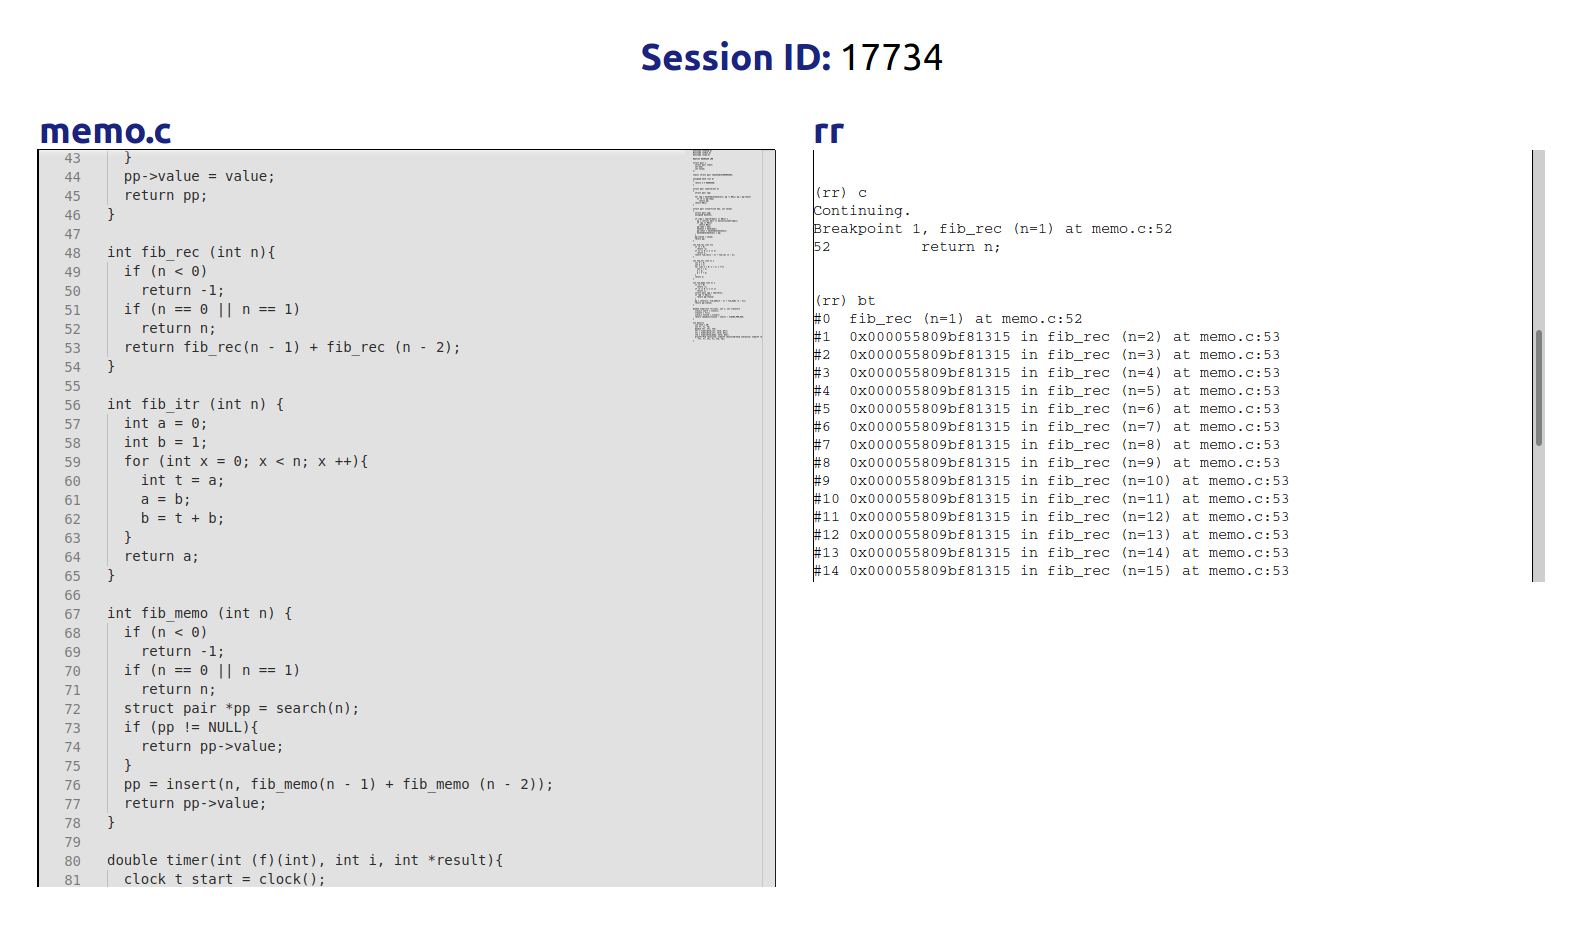
\includegraphics[width=\textwidth]{memoization}
  \centering
  \caption{Debugging the Memoization Example Session}
  \label{frontend:rrterm}
\end{figure}

\begin{enumerate}
\item Students A and B both log into the collaborative debugger from
  different computers.
\item Student A creates a new Debug Session by clicking the button for
  \lstinline{memoization} under ``New Session''.  A few moments later,
  they're presented with the main screen of the debugger.
\item Using the session code (17734 in the example above), Student B
  joins the Debug Session.
\item Both students can now interact with the same debugger remotely.
  Input and output from the debugger and the current source file are
  synced between all students.  Students can work together to
  understand the reasons why memoization often improves the execution
  time of recursive programs.
\end{enumerate}

\subsection{Tools Used}

The frontend of the collaborative debugger must handle constant
changes in state as users participate in the process outlined above.
The frontend uses React, Monaco, and Xterm.js to manage state and
display output.  It primarily displays the output from rr, an
enhancement of gdb that the collaborative debugger uses to enable
collaboration.

\subsubsection{Mozilla's rr}\label{rr}

Notice that the debugging window in the above example is called
``rr''. rr is ``a lightweight tool for recording, replaying and
debugging execution of applications''\cite{rr-repo}. rr allows a
programmer to record the execution of a program on any compatible
machine and replay the execution later.  This enhances GDB's ability
to ``time-travel'' when debugging, using commands such as
\lstinline{reverse-continue} and
\lstinline{reverse-stepi}\cite{gdbman} to step backwards and forwards
through a program's execution.  Through a novel encapsulation of the
execution space, rr is able to deterministically record and replay the
execution of syscalls and other process behavior that differs
run-to-run.  This is invaluable when trying to debug behavior that is
not entirely dependent on the code being debugged.  A typical workflow
in rr consists of recording an inexplicable error, replaying execution
to find the area in which the error occurs, and then narrowing in on
the bug not by re-running the entire program, but by progressing back
and forth through execution in the problem area.
\par

rr is an ideal tool for teaching debugging because it allows
instructors to record execution of a program and design a debugging
example with the knowledge that normally non-deterministic events will
be repeatable, and that any input they provide to the program will be
exactly replicated.  With the collaborative debugger, teachers can
record a program's execution and design a debugging lesson which
students can work on together.  The repeatability of rr means that
students can focus on debugging, and teachers can create as specific
examples as they please.  The use of rr is the most significant step
the collaborative debugger takes to addressing the lack of
back-tracing ability/coverage found in existing tools for teaching
debugging\cite{10.1145/3286960.3286970}.

In comparison to solutions like PANDA\cite{10.1145/2843859.2843867}
that rely on capturing the entire state of of a virtual machine to
replay execution, rr records and replays faster, produces far smaller
files, and doesn't force execution inside of a
VM.\cite{DBLP:journals/corr/OCallahanJFHNP17} The trade off for these
benefits are two major system limitations: rr is only compatible with
the Linux kernel, and it's deterministic recording and replay relies
on a feature that is only found on modern \textit{Intel} x86 CPUs.
These limitations influenced the development of this project as a
webapp similar to existing tools for collaborative programming.
\par

Luckily, the speed and size benefits of rr lend themselves well to
non-local execution.  In conjunction with tools used to create the
backend of the collaborative debugger it takes a few seconds to create
a new debug session running rr and connect it to the frontend webapp
discussed in this section.

\subsubsection{React}\label{react}

React is JavaScript library that simplifies creating user interfaces
and managing state \cite{react}.  React's state management is of
particular importance to the collaborative debugger's frontend.  State
constantly changes as users create/delete debugging sessions, join
existing sessions, and communicate with rr.  React allows classes and
functions to encapsulate components such as a list of existing
debugging sessions, a view of the current program's source code, and
the terminal interface with rr.  Instances of these classes maintain
state and update efficiently.
\par

The frontend makes extensive use of JSX, syntax which allows the
inclusion of segments of HTML code within a React app written in
JavaScript.  This makes it easy for each component of the one-page
webapp to hide/show subcomponents as state changes.

\subsubsection{Monaco and Xterm.js}\label{xtermjs/monaco}

After joining or creating a debugging session, users spend most of
their time interacting collaboratively with rr.  Their primary
interface to rr is through Xterm.js, a frontend component that makes
it easy to emulate terminal behavior in the browser \cite{xtermjs}.
With a few control methods, it is simple to provide a terminal
interface to rr that is virtually indistinguishable from a local
session.  By using the Xterm.js based interface, students can learn to
use rr (and by extension gdb) collaboratively, and directly translate
that knowledge to individual work.
\par

In addition to the terminal interface, the frontend shows a view of
the current source file being debugged.  The Monaco Editor
\cite{monaco} is used to display this source view.  Though more
complex than is strictly necessary to display code, Monaco makes it
easy to format and syntax-highlight.  Using Monaco also simplifies the
future addition of editing source code, should the need arise.
React's state management allows updating text in the editor as
efficiently as possible.

In order to easily integrate Monaco and Xterm.js into the React
frontend, React wrapper libraries were used.  These are
react-xterm\cite{reactxterm} and
react-monaco-editor\cite{reactmonaco}.

\subsection{Overview}

% The frontend webapp communicates with a distributed backend.  A simple
% diagram of the entire system is below.

% \begin{figure}[h!]

%   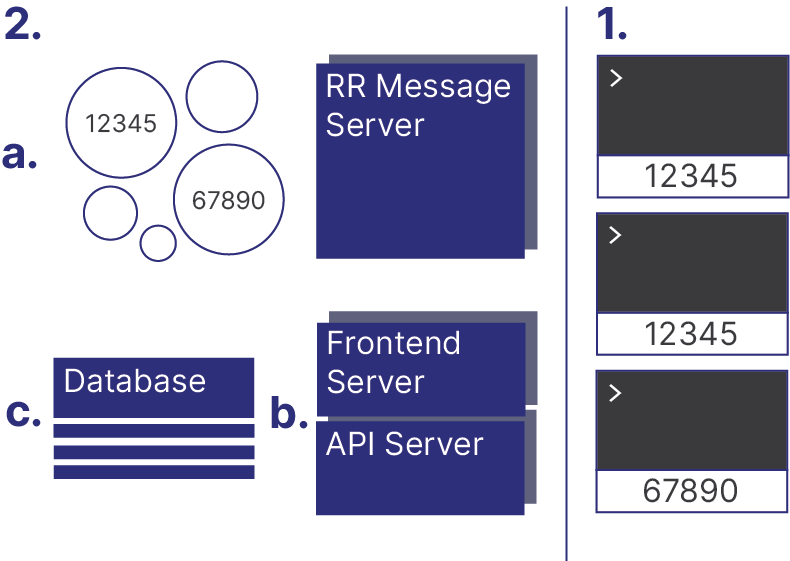
\includegraphics[scale=.8]{overall_system}
%   \centering
%   \caption{Overview of the Collaborative Debugger}
%   \label{debugger:overview}
% \end{figure}

% The collaborative debugger consists of:

% \begin{enumerate}
% \item A frontend web app that presents a debugging interface to the
%   end user.
% \item A distributed backend split into three parts:
%   \begin{enumerate}
%   \item 
%   \item Pods running a frontend server written in Node.js which works
%     in tandem with an API server created using Flask
%     (\ref{flask/node}).  The API server manages creation and
%     destruction of debug sessions, as well as authentication.
%   \item A MongoDB (\ref{mongodb}) database.
%   \end{enumerate}
% \end{enumerate}

React makes it easy to create simple webapps with no build
configuration necessary through the use of the
\lstinline{create-react-app} command.  This creates a structure and
toolchain for a basic one-page application---suitable for the
collaborative debugger.  Once this structure was created and any
superfluous files/code were removed, it wasn't necessary for the
purposes of the collaborative debugger to directly edit any files
except two: \lstinline{App.js} and \lstinline{App.css}.  The
pre-defined build process takes care of transforming the React code
defined in \lstinline{App.js} and the styles defined in
\lstinline{App.css} into portable JavaScript, HTML, and CSS.
\par

\lstinline{App.js} consists of a primary React Component class,
\lstinline{Debugger}, as well as many secondary classes and functions.
More complex components of the frontend, such as the Xterm.js
interface to rr, are created as classes, while simple components like
buttons are defined as functions.  All classes contain a
\lstinline{render()} method responsible for returning HTML elements to
display based on the state contained in the class.
\lstinline{Debugger}'s \lstinline{render()} method is responsible for
displaying all other components, based on whether the user is logged
in, has selected a new session, etc.
\par

Many components ``lift state up'' to \lstinline{Debugger}.  This is
accomplished by passing methods from \lstinline{Debugger} in as
``props'' when elements are created in \lstinline{Debugger}'s
\lstinline{render()} method:

\begin{lstlisting}[language=Javascript,basicstyle=\linespread{0.5}\ttfamily,caption={Lifting State Up},captionpos=b]
  onLogin(name) {
    this.setState({user: name})
    .
    .
    .
  }
  // In Debugger.render().  This is JSX.
  login = <LoginForm onLogin={this.onLogin}/>;
  
  // In LoginForm.
  this.props.onLogin(data.name);
\end{lstlisting}

\lstinline{Debugger}'s \lstinline{onLogin(name)} method changes the
state of debugger to indicate that the user is logged in.  When an
instance of \lstinline{LoginForm} is created in
\lstinline{Debugger.render()}, \lstinline{onLogin(name)} is passed to
it as a ``prop''.  The code for logging in the user can be contained
in \lstinline{LoginForm}, but when it becomes necessary to change the
state of the whole application to indicate that the user is logged in,
\lstinline{LoginForm} calls \lstinline{Debugger.onLogin(name)},
lifting state up to \lstinline{Debugger}.
\par

Other than methods to handle state and display components,
\lstinline{Debugger} also contains the Socket.IO client that is used
to communicate with the actual debugger running in the collaborative
debugger's backend.  Socket.IO is a library that extends WebSockets.
It and this communication process will be discussed in detail in
(\ref{rrmessageserver}).  Similarly to how \lstinline{onLogin(name)}
is passed as a property to \lstinline{LoginForm}, the Socket.IO client
is passed to the most important component in the frontend,
\lstinline{RRTerm}, when it is instantiated.

\subsection{The Collaborative Interface to rr}

As shown in Figure \ref{frontend:rrterm}, the primary piece of the
collaborative debugger's frontend is an interface to the rr debugger
backend.  This interface currently consists of a view of the user's
source code and a terminal interface to rr.  These are contained
within the most important class in the frontend: \lstinline{RRTerm}.
This section will outline the process of sending an rr command to the
backend and displaying a response.  Apart from sending simple API
requests to start sessions or log users in and out, this communication
process is where the frontend webapp spends most of its time.
\par

In debugging the \lstinline{memoization} example program, users will
want to display the call stack from within each implementation of the
nth Fibonacci number function.  To stop in \lstinline{fib_rec}, the
recursive implementation, one user will want to set a breakpoint at
line 52 in the source file.  To do this they will type the command
\lstinline{break 52} and hit enter.  The command will be sent to the
backend, and all users in the same debug session (17734 in Figure
\ref{frontend:rrterm}) will see the debuggers response:\\
\lstinline{Breakpoint 1 at 0x561c8fede303: file memo.c, line 52.}\\
Users who did not send the command \lstinline{c} will see it displayed
along with the response.

\subsubsection{Sending a Command}

\lstinline{RRTerm}'s state is instantiated as such:

\begin{lstlisting}[language=Javascript,basicstyle=\linespread{0.5}\ttfamily,caption={RRTerm's State},captionpos=b]
  this.state = {command: '',
                  name: '',
                  linum: 0,
                  code: ''};
\end{lstlisting}

\lstinline{name}, \lstinline{linum}, and \lstinline{code} store
information about the current source file being debugged.
\lstinline{command} is the most important field for examining how
commands are sent to the backend, as it holds the current command.
\textit{Every time} the user types a character, \lstinline{command} is
updated to reflect the current state of the Xterm.js component.  The
code to handle keystrokes is shown below:

\begin{lstlisting}[language=Javascript,basicstyle=\linespread{0.5}\ttfamily,caption={Handling Keystrokes},captionpos=b]
  this.term.on('key', (key, ev) => {
    const printable = !ev.altKey && !ev.ctrlKey && !ev.metaKey;
    if (ev.key === 'Enter') {
      // Disable input while we wait for the response from rr
      this.term.disableStdin = true;
      const c = this.state.command;
      this.sendCommand(c);
      this.setState({command: ''});
    } else if (ev.key === 'Backspace') {
      // Do not delete the prompt
      if (this.term.buffers._activeBuffer.x > prompt_length) {
        this.term.write('\b \b');
        this.updateCommand(this.state.command, 'delete');
      }
    } else if (ev.key === 'ArrowUp') {
    } else if (ev.key === 'ArrowDown') {
    } else if (printable) {
      this.term.write(key);
      this.updateCommand(this.state.command, key);
    }
  });
\end{lstlisting}

Whenever the user types a printable key, the key is written to the
terminal and \lstinline{command} is updated using the
\lstinline{updateCommand} method.  If a user types \lstinline{brk},
\lstinline{updateCommand} would be called three times, once for each
keystroke.  Upon realizing they made a mistake when typing
\lstinline{break 52}, the user would likely delete a character.  As
long as the prompt (\lstinline{(rr)} followed by a space) would not be
overwritten, the terminal is updated and \lstinline{updateCommand} is
called again.  When the user hits the enter key the command is finally
sent to the backend using \lstinline{sendCommand}.  To mimic the
behavior of a local rr debug session and to prevent garbled input,
writing to the terminal is disabled until a response is received.

\subsubsection{Receiving a Response}

All users connected to the same debug session will receive responses
to the commands sent by one user.  This is how collaboration is
achieved in the collaborative debugger.  The JSON response object to
\lstinline{break 52} received by all users is shown below:

\begin{lstlisting}[basicstyle=\linespread{0.5}\ttfamily,caption={JSON Response},captionpos=b]
{
  channel: ``11734''
  command: ``break 52''
  from: ``1ed644ad87d44cd68121de3daa65adb4''
  response: {
    output: ``Breakpoint 2 at 0x561c8fede303: file memo.c, line 52.''
    source: {
      file_name: null
      current_line: ``87''
      contents: null
    }
  }
}
\end{lstlisting}

The command has been issued from a breakpoint set at \lstinline{main},
which is at line 87 in \lstinline{memo.c}.  Since the source file
hasn't changed, \lstinline{source.file_name} and
\lstinline{source.contents} are set to \lstinline{null}.
\lstinline{output} contains the response from rr, while
\lstinline{channel}, \lstinline{command}, and \lstinline{from} contain
information necessary to display commands correctly for all users.

\begin{lstlisting}[language=Javascript,basicstyle=\linespread{0.5}\ttfamily,caption={Processing a Response},captionpos=b]
  this.props.socket.on('rr_response', (data) => {
    if(data.from !== this.props.socket.id){
      // Display commands from other clients
      this.term.disableStdin = true;
      this.term.clear();
      this.term.write(data.command);
    };
    // Write a newline, but no prompt
    this.term.writeln('');
    // Write each line of the output to the terminal
    data.response.output.split(/\n+/).forEach((l) => {
      this.term.writeln(l);
    });
    this.term.prompt();
    // Re-enable input.  See above and below.
    this.term.disableStdin = false;
    // If an error has occured, there wont be any new
    // information about the location in the source file.
    if(data.response.source != null) {
      this.updateSource(data.response.source);
    }
  });
\end{lstlisting}

When a response is received, \lstinline{RRTerm} first checks to see if
the response has originated from a different user.  If so, input is
disabled, the current line is cleared, and the command that
corresponds to the response is written to the terminal.  Each line of
the response is then written to the terminal.  Finally, input is
renabled, having been disabled either to write commands received from
another user, or when the command was first sent.
\lstinline{updateSource} is called to update the Monaco editor source
file view.  Since \lstinline{break 52} was sent from a location
already inside \lstinline{memo.c}, the source file name and contents
are not updated, though the line number is changed.

\subsection{Considerations} \label{vistools}

The intention of much of the code described above, such as that to
disable input after a command has been sent, is to mimic rr in a way
that is invisible to the user.  The user experience is intended to be
that of using a fully-fledged debugger collaboratively.  The source
code view allows users to easily see what code they are working on
together, and the terminal updates quickly whenever a user enters a
command.
\par

Care has been taken to design the frontend in a modular fashion so
that it can be easily extended in the future.  Visualization tools
could be easily added by sending additional data about program state
in the response and creating new components.  If further
authentication features or the ability to edit source code are desired
in the future, relevant components can be updated without the need to
change the entire application.  Since the collaborative debugger
depends heavily on interactions between its frontend and backend,
similar care has been taken in designing the backend, which will be
described in the following sections.

\section{Backend Design Overview}

The design of the collaborative debugger's backend is heavily
distributed, allowing individual components to be modified without the
whole system needing to be reconfigured.  Kubernetes in conjunction
with Docker are used to create the backend of the collaborative
debugger.

\subsection{Tools Used}

Kubernetes and Docker were chosen largely so that new Debug Sessions
could be easily and securely created on demand.

\subsubsection{Docker}\label{docker}

Docker is containerization software.  Docker containers encapsulate
applications and their dependencies while sharing their host's kernel.
This allows for lightweight, portable, and secure execution of complex
programs \cite{docker}.  All programs in the collaborative debugger's
backend run in Docker containers.  Docker containers' lightweight
nature and security are instrumental when trying to quickly create
containers to run user-defined code.

\subsubsection{Kubernetes}\label{k8s}

Kubernetes is the de facto standard in container orchestration
software.  It provides a layer of abstraction on top of normal
containers, like those created by Docker.  By bundling one or more
closely linked containers into a ``Pod'', Kubernetes is able to manage
deployment and re-deployment of applications running inside
containers.  It is trivial to create new Pods (or multiple Pods
running the same application) as needed within a Kubernetes cluster
\cite{k8s}.  The speed at which even relatively large Pods can be
created and the inherent security provided by containerization drove
the decision to create a new Pod on the fly for each debugging
instance in the collaborative debugger.  This allows the debugger to
provide a similar level of convenience to existing collaborative
tools, such Replit (\ref{exisitingcollab}).
\par

Kubernetes also provides services to facilitate load balancing, manage
storage volumes, and contain secrets.  The abstraction provided by
these features, in tandem with the ease of Kubernetes deployment on a
managed Kubernetes service\cite{do_managed_k8s} greatly accelerated
development.

\subsection{Overview}

The collaborative debugger consists of a distributed Kubernetes
backend and frontend React webapp.  Kubernetes was chosen for the
backend primarily so that a Pod could be created dynamically for each
debugging session.  

\begin{figure}[h!]

  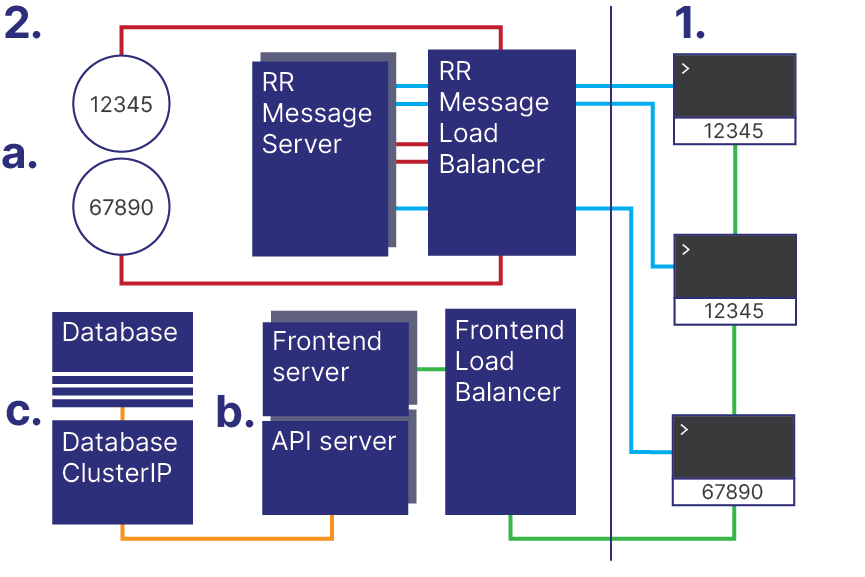
\includegraphics[scale=.9]{detailed_system}
  \centering
  \caption{Detailed Overview of the Collaborative Debugger}
  \label{debugger:detailedoverview}
\end{figure}

Each backend component of the collaborative debugger runs in it's own
individual Pod.  There are two different classes of Pods in the
collaborative debugger:

\begin{enumerate}
\item Statically created Pods.  These are the \textit{RR Message
    Server Pods}, the \textit{Frontend/API Server Pods}, and the
  \textit{Database Pod}.  This class of Pods are manually created when
  the cluster that will run the backend is first initialized.  The RR
  Message Server Pods and Frontend/API Server Pods may be created
  using Deployments \cite{k8s_docs} to allow scaling, where multiple
  Pods running the same application may be created to facilitate
  increased load.
\item Dynamically created Pods.  This class of Pod contains the
  individual instances of \textit{RR Debug Session Pods} that are
  created on request by the API server.  When a client requests a new
  debug session, the API server uses the Kubernetes API to create a
  new Pod based on an existing template, gives the Pod a unique
  identifier, and associates it in the database with the requesting
  client.
\end{enumerate}

These Pods communicate with other Pods in the cluster and with the
outside world through Services.  The Kubernetes documentation defines
a Service as ``an abstraction which defines a logical set of Pods and
a policy by which to access them'' \cite{k8s_docs}.  In the
collaborative debugger, these Services manifest as:

\begin{enumerate}
\item The \textit{Database ClusterIP}: a ClusterIP, which exposes the
  Database Pod only inside the cluster.  The only component that makes
  use of this ClusterIP is the API server, which uses it primarily to
  communicate information about users and RR Debug Sessions with the
  database.
\item The \textit{RR Message Load Balancer}: a Load Balancer, which
  exposes the RR Message Server Pods to the outside world.  Using
  Socket.IO, clients send commands to and receive responses from
  individual RR Debug Session Pods through the RR Message Server Pods.
\item The \textit{Frontend Load Balancer}: another Load Balancer,
  which exposes the Frontend/API Server Pods to the outside world.
  Clients request the frontend webapp and send API requests/receive
  API responses through this Load Balancer.
\end{enumerate}

The frontend webapp dynamically updates as the user requests new debug
sessions, issues commands to rr, and visits new source files.  A user
can be part of multiple debug sessions simultaneously.  Each debug
session is assigned at 5 digit identifier at creation, which is used
to join sessions in progress.
\par

Each component of the backend will be discussed in depth in the
following sections.

\subsection{Configuration and Setup}

Configuration and setup of the collaborative debugger is relatively
simple.  After a Kubernetes cluster is created (this is made easier by
using a Managed Kubernetes service) Pods and Services are created
using various configuration files.  Services should be created first,
so that Pods which rely on access to Services function properly on
creation.  The following sections outline the process of creating a
cluster, Pods, and Services, with a focus on statically created Pods.
The process of building images for building dynamically created Pods
is similar, but the process of starting the Pods is more complicated.
This process will be discussed in-depth in the section on the API
server (\ref{api}).

\subsubsection{Cluster Requirements and Configuration}

Though Kubernetes aims to be largely platform-agnostic, the
requirements of rr impose some restrictions on cluster setup and
configuration.  Clusters, even those running inside a VM, must be run
on machines using relatively modern Intel x86 CPUs (Nehalem and
beyond).  The clusters must run on an operating system using Linux
kernel version 3.11 or higher \cite{rr-repo}.  Finally, in order for
rr to be able to work efficiently, the
\lstinline{kernel.perf_event_paranoid} parameter must be set to
\lstinline{1} \cite{rr-repo}.  This should be done on every node in
the cluster which will run RR Debug Sessions.  For the purposes of
development, it has been set to \lstinline{1} on all nodes in the
collaborative debugger cluster.

\subsubsection{Creating Pods}

\begin{figure}[h!]

  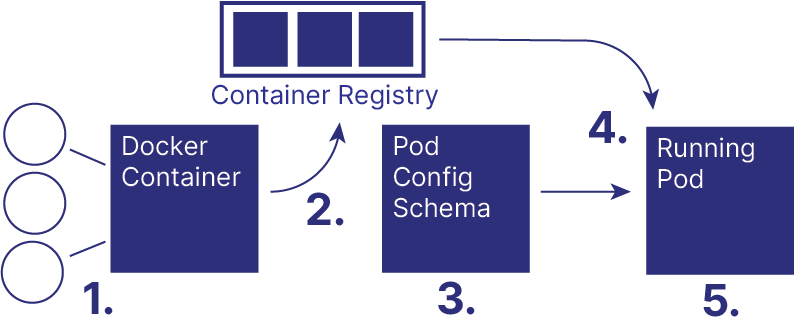
\includegraphics[scale=.9]{pod_creation}
  \centering
  \caption{The Pod Creation Process}
  \label{podcreation:overview}
\end{figure}

Pods are created in five steps:

\begin{enumerate}
\item A \lstinline{Dockerfile} is used to build a new Docker container
  image from various pieces of source code, scripts, and a base image
  (such as the official MongoDB image or official Ubuntu image).  The
  Dockerfile also contains instructions to install necessary packages,
  run build scripts, and create file structures in the image.
\item The Docker image is tagged and uploaded to a private container
  registry.
\item A Pod configuration schema is defined/updated with details of
  the corresponding image's tag and any necessary Pod-specific
  settings/startup commands.
\item The Pod configuration schema is applied, either statically or
  dynamically.  When the schema is applied, Kubernetes pulls the image
  from the container registry and creates a new Pod according to the
  schema, running any startup commands if provided.
\item If Pod creation is successful, the result is a new Pod running
  in the cluster.
\end{enumerate}

\paragraph{1. Docker Container Creation}

Docker containers are created using a Dockerfile.  The Dockerfile used
to create the container image for the RR Message
Server is shown below:

\begin{lstlisting}[language=Dockerfile,caption={RR Message Server Dockerfile},captionpos=b]
# Base Image
FROM  ubuntu:latest

# Package Installation
WORKDIR /tmp/
ENV DEBIAN_FRONTEND="noninteractive"
RUN apt-get update && apt-get install -y \
python3-pexpect python3-pip

# User Creation
RUN useradd -ms /bin/bash rrserver
USER rrserver

# File structure creation/app setup
RUN pip3 install requests python-socketio \
eventlet
WORKDIR /home/rrserver/
RUN mkdir app
WORKDIR /home/rrserver/app/
COPY server.py .
COPY startup.sh .

# Startup command
CMD ["sh", "startup.sh"]
\end{lstlisting}

The build process for each collaborative debugger Docker image follows
the same structure as the one outlined in the Dockerfile above:

\begin{enumerate}
\item The base image is defined. The RR Message Server and RR Debug
  Session images are based on the latest Ubuntu image.  This is
  particularly necessary for the RR Debug Session image, as rr's
  low-level nature necessitates somewhat frequent updates as changes
  are made to the Linux kernel.  The Frontend/API Server image is
  based on the latest Node image, and the Database image is based on
  the latest MongoDB image.
\item Second, any necessary packages are installed.  For the RR Debug
  Session image, rr is compiled from source and installed.
\item A non-root user is created if necessary.
\item Program files are copied over and a file structure is created.
  Packages that don't rely on the base image's built in package
  manager are installed at this time.  In the example above, these
  include Python packages.
\item A startup command is defined.
\end{enumerate}

Each line in a Dockerfile corresponds to a layer in the built image.
This build order minimizes the amount of rebuilding necessary by
placing the items that are most likely to change towards the end of
the build process.

\paragraph{2. Container Registry Upload}

Most Managed Kubernetes services come with the option to create a
private container registry.  With proper authentication, this allows
Docker and Kubernetes to access user-created images as easily as if
they were in a public registry.  Images built with Docker are uploaded
to a private container registry for use in the collaborative debugger.

\paragraph{3. Pod Configuration Schema} \label{podschema}

The Pod configuration schema for most Pods in the collaborative
debugger is fairly generic.  It consists of a \lstinline{name}, an
\lstinline{image} sourced from the container registry, and in the case
of pods that need to interact with a load balancer, an
\lstinline{app}.

\begin{lstlisting}[language=YAML,basicstyle=\linespread{0.5}\ttfamily,caption={RR Debug Session Schema},captionpos=b]
apiVersion: v1
kind: Pod
metadata:
  name: rr-translation
  labels:
    purpose: translate-rr
spec:
  containers:
  - name: rr-test-container
    image: example-container-registry.com/sproj/...
    securityContext:
      capabilities:
        add:
        - SYS_PTRACE
  restartPolicy: OnFailure
\end{lstlisting}

A notable exception is the RR Debug Session Schema, which adds the
\lstinline{SYS_PTRACE} capability to the Pod.  This is necessary for
rr to properly trace system calls.

\paragraph{4 \& 5. Pod Creation}

For statically created Pods, the \lstinline{kubectl apply} command is
used to create new Pods.  Kubernetes pulls the container image defined
in the schema from the container registry and starts the Pod with any
necessary commands.  The database Pod is connected to a long-term
storage volume at this time.  Upon successful creation, the Pod is
ready to interact with any necessary load balancers.

\subsubsection{Service Creation}

Services are the first components of the collaborative debugger
created after the cluster is initialized.  The three Services used by
the debugger are all statically created.  Like statically created
Pods, schemas that define Services are applied manually using the
\lstinline{kubectl apply} command.

\begin{lstlisting}[language=YAML,basicstyle=\linespread{0.5}\ttfamily,caption={Frontend Load Balancer Schema},captionpos=b]
apiVersion: v1
kind: Service
metadata:
  name: frontend-load-balancer
spec:
  selector:
    app: frontend
  type: LoadBalancer
  ports:
    - port: 3000
    targetPort: 3000
\end{lstlisting}

The \lstinline{app} field in the above schema corresponds to the
\lstinline{app} field defined in the metadata of the Frontend/API
Server configuration schema.  Traffic to the Load Balancer's external
IP address on port 3000 is redirected automatically by Kubernetes to
any Pod running the Frontend/API Server.  The Load Balancer determines
which Pod is the most suitable given current demands on the system.

\section{RR Debug Sessions \& RR Message Server}

At the heart of the collaborative debugger is the RR Debug Session.
Every time a user wants to debug a new program execution, an RR Debug
Session Pod is dynamically created by the API server.  The new Pod is
assigned a unique five digit identification number when it is created.
This five digit number is used as the channel for the RR Debug
Session, separating its communication from other RR Debug Session
Pods.  Clients, RR Message Server Pods, and the RR Debug Session Pod
connect through the RR Message Load Balancer.  Clients and RR Debug
Sessions send messages using the channel assigned to the pod at
creation time.  A diagram of one full communication cycle between two
clients and an RR Debug Session Pod is outlined in the diagram below:

\begin{figure}[h!]

  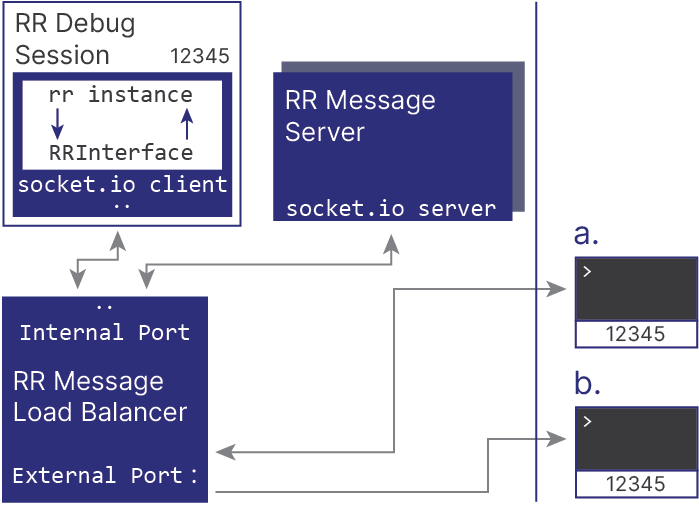
\includegraphics[scale=.8]{rr_detailed}
  \centering
  \caption{RR Message Server Communication Cycle}
  \label{rr:detailed}
\end{figure}

The process of sending a command to an RR Debug Session and receiving
a response is as follows:

\begin{enumerate}
\item Client A, already having connected to the channel that
  corresponds to it's current RR Debug Session (channel 12345 in the
  example), sends an rr command.
\item The RR Message Server receives the command and emits a message
  that RR Debug Session Pods are equipped to receive on the same
  channel.  In practice, since only one RR Debug Session Pod is ever
  on a channel, this equates to emitting a message to the Pod
  directly.
\item The RR Debug Session Pod receives the message, and passes the
  command to its instance of RRInterface, the class which controls rr.
  When it receives a response, it emits the output from rr along with
  other debugging information and the channel.
\item The RR Message Server receives the response, and emits a
  response message that clients are equipped to receive on the
  corresponding channel.
\item Clients A and B are connected to the corresponding channel, so
  they both receive the response.
\end{enumerate}

\subsection{RR Message Server}\label{rrmessageserver}

\subsubsection{Tools Used}

The collaborative debugger needs an efficient way for clients to
communicate with running RR Debug Sessions. The Socket.IO library was
selected to construct this efficient communication pathway.

\paragraph{Socket.IO}\label{socketio}

To speed communication, the collaborative debugger uses WebSockets to
directly connect web clients and the Pods running rr.  Socket.IO is a
library that extends WebSockets.  It provides backup in case a
WebSocket connection cannot be established, enables automatic
reconnection and disconnection detection, and adds support for
namespaces \cite{socketio}.  The collaborative debugger uses the
standard JavaScript implementation of Socket.IO on the client side.
Messages are passed through a server to individual debugging Pods,
both of which use the Python implementation of Socket.IO,
python-socket.io \cite{python_socketio}.

\subsubsection{Overview}

The RR Message server is remarkably simple, consisting of just 3
important functions:

\begin{lstlisting}[language=Python,basicstyle=\linespread{0.5}\ttfamily,caption={RR Message Server},captionpos=b]
@sio.on('join_channel')
def join_channel(sid, data):
    sio.enter_room(sid, data['channel'])

@sio.on('rr_command')
def on_rr_command(sid, data):
    data['sid'] = sid
    try:
        sio.emit('rr_command', data,
                 room=data['channel'])
    except:
        pass

@sio.on('rr_response')
def on_rr_response(sid, data):
    sio.emit('rr_response', data,
             room=data['channel'])
\end{lstlisting}

Even in a fully production ready version of the collaborative debugger
with more security features enabled, the RR Message Server is unlikely
to become much more complex.  It exists purely to pass messages
between clients and RR Debug Session Pods and to manage channels.
Since the design of other aspects of the collaborative debugger ensure
that all members of a given channel exist only during the lifetime of
it's corresponding RR Debug Session Pod, the
\lstinline{'join_channel'} event handler simply adds socket.io clients
to a specified channel on request.
\par

The two message processing functions, \lstinline{on_rr_command} and
\lstinline{on_rr_response}, are equally simple.  When the RR Message
Server receives an \lstinline{'rr_command'} message, it passes the
message data along to the corresponding RR Debug Session Pod by
emitting an \lstinline{'rr_command'} namespaced to the correct channel
with \lstinline{room=data['channel']}.  Since the socket.io client
running in RR Message Server Pods has an event handler defined for
\lstinline{'rr_command'}s but frontend clients do not, only RR Message
Server Pods receive the command.  The same process happens in reverse
for \lstinline{'rr_response'}s, with only the frontend socket.io
clients having a handler defined for \lstinline{'rr_response'}.

\subsection{RR Debug Session} \label{rrpods}

\subsubsection{Tools Used}

RR Debug Sessions primarily manage and communicate with rr, which has
already been covered in detail in \ref{rr}.  pygdbmi is used for this
process.

\paragraph{pygdbmi}

In order to ``support the development of systems which use the
debugger as just one small component of a larger system'', gdb
provides a machine-oriented interface called gdb/mi \cite{gdbman}. rr
supports interaction through gdb/mi, and using the interface was a
natural choice for the collaborative debugger.  In addition to being
far easier to interact with from within a program, the structured,
machine-friendly output of gdb/mi lends itself in particular to future
development of visualization aids in the collaborative debugger.
\par
To parse rr output into Python dictionaries and to easily control rr
as a subprocess, pygdbmi \cite{pygdbmi} is used in each debugging Pod.
pygdbmi's abstraction simplifies programmatically controlling rr.  A
Pod can receive a command from the client, pass it to rr, and respond
without having handle directly parsing gdb/mi output or managing the
rr process.

\subsubsection{Building Example Pods} \label{buildingchannel}

The process for building RR Debug Session example images is differs
slightly from other images used by the collaborative debugger.
Currently, three example RR Debug Session images are available for
use: \lstinline{hash}, \lstinline{smash}, and \lstinline{memoization}.
Example container images are based on the primary RR Debug Session
image, RR Translation.  The build process for this image, based on the
lasted official Ubuntu container image, installs rr, python, and all
necessary packages as well as the app that will run on the final
image, \lstinline{rrtranslation.py}.

\begin{lstlisting}[language=Dockerfile,basicstyle=\linespread{0.5}\ttfamily,caption={RR Debug Session Hash Example---Dockerfile},captionpos=b]
FROM example-container-registry.com/sproj/...
  
WORKDIR /home/debug/app/
COPY hash.c .
COPY names .
COPY startup.sh .
\end{lstlisting}

The Dockerfile shown above is for the \lstinline{hash} RR Debug
Session example.  The build process copies over any necessary files,
as well as a startup script:

\begin{lstlisting}[basicstyle=\linespread{0.5}\ttfamily,caption={Example Startup Script},captionpos=b]
gcc -g -o hash hash.c
rr record ./hash
python3 rrtranslation.py $1
\end{lstlisting}

This script is used to start the \lstinline{'rrtranslation.py'} program
when the Pod is dynamically created.  The script will be passed the
Pod's channel as argument \lstinline{$1} by the Kubernetes API on
startup.
\par

Current example pod startup scripts compile the program to be debugged
and record execution when the pod is created.

\subsubsection{The RR Translation Program} \label{joiningchannel}

The RR Translation program consists of two main components: a
Socket.IO client, \lstinline{sio}, and an instance of the
\lstinline{RRInterface} class, \lstinline{rri}, that controls the rr
subprocess and parses interactions.  Simple code to read information
about the current source file currently exists within
\lstinline{sio}'s \lstinline{'rr_command'} event handler, but should
be broken out into its own class if more complexity is added.
\par

The RR Translation program's socket.io client instance begins by
connecting to the RR Message Server.  It immediately emits a
\lstinline{'join_channel'} message, using the channel number passed in
by the Kubernetes API on Pod creation (\ref{dynamicc}).

\begin{lstlisting}[language=Python,basicstyle=\linespread{0.5}\ttfamily,caption={RR Translation Main},captionpos=b]
if __name__ == '__main__':
    channel = sys.argv[1]
    sio.connect('http://rr-message-server-load-balancer:8000')
    sio.emit('join_channel', {'channel': channel})
\end{lstlisting}

After joining the appropriate channel, \lstinline{sio} waits to
receive an \lstinline{'rr_command'}.  The first part of
\lstinline{sio}'s \lstinline{'rr_command'} event handler is shown below:

\begin{lstlisting}[language=Python,basicstyle=\linespread{0.5}\ttfamily,caption={RR Command Event Handler},captionpos=b]
@sio.on('rr_command')
def on_rr_command(data):

    body = {'from': data['sid'],
            'command': data['command'],
            'channel': channel}
    
    try:
        response = {'output': rri.write(data['command'])}
\end{lstlisting}

The handler first builds part of the response body, passing back data
about the channel and originator of the message that will be important
for the RR Message Server and client later.  Next, it calls the
function necessary to pass a message to rr and receive a response,
\lstinline{rri.write()}.
\par

When the program starts, an instance of the \lstinline{RRInterface}
class, \lstinline{rri}, is initialized in the same scope as
\lstinline{sio}.  \lstinline{RRInterface} contains an instance of the
\lstinline{gdbController} class from pygdbmi to interface with rr and
control the rr subprocess, as well as a collection of methods to parse
rr output, the three most important of which are shown below: 

\begin{lstlisting}[language=Python,basicstyle=\linespread{0.5}\ttfamily,caption={RRInterface},captionpos=b]
def get_full_rr_response(self, command):
    response = self.gdbmi.write(command)
    while(not(self.end(response) or self.exited(response))):
        response.extend(self.get_rr_response())
    return response

def write(self, command):
    if self.command_forbidden(command):
        raise DissallowedError
    self.timeline.append(command)
    return self.console_output(
        self.get_full_rr_response(command))

def source(self):
    f = self.get_full_rr_response(
        '-file-list-exec-source-file')[0]['payload']
    return {'file': f['file'],
            'line': f['line'],
            'path': f['fullname']}
\end{lstlisting}

When \lstinline{write} is called, it determines if the command to be
executed is forbidden.  Currently only one gdb command,
\lstinline{shell}, is disallowed.  Parsing the output from
\lstinline{shell} is difficult, it is of virtually no use since
\textit{recordings}, not currently executing programs that
\lstinline{shell} could effect, are being debugged.  It also opens the
door to security issues.  Though containerization means that the most
users could probably do is render their own debug session useless, the
downsides of \lstinline{shell} far outweigh the benefits.
\par

Next, write appends the command to the \lstinline{RRInterface}'s
\lstinline{timline} instance variable.  \lstinline{timeline} is a list
of all commands the debug session has executed.  Though unused at the
moment, it can serve in the future to implement a shared history
between all clients and to facilitate the saving of debug sessions
in-progress.  By issuing all commands in \lstinline{timeline} to a new
instance of \lstinline{RRInterface} with the same recording, it is
possible to restore a debug session to an identical previous state.
To save a debug session, the recording and \lstinline{timeline} can be
stored in a database, and be used to initialize a new Pod with
identical state to a previous RR Debug Session Pod.  This appears to
clients as a seamless restoration of a previous Debug Session.
\par

Since the frontend currently consists of a terminal interface to rr
and a view of the current source code, \lstinline{write} does not need
to return any information from rr other than console output.  Future
versions of the collaborative debugger that support visualization
tools could use gdb/mi commands such as \lstinline{-stack-list-frames}
to retrieve information to be used by frontend visualization tools.
\lstinline{console_output} extracts user-relevant output from the
dictionary returned by \lstinline{GDBController}'s \lstinline{write}
method.  The \lstinline{get_full_rr_response} method ensures that all
relevant output has been received from the rr subprocess before
returning.  \lstinline{write} reduces the lengthy dictionary that
would be produced by a command as simple as \lstinline{break main}
into a few lines of user-relevant output.
\par

After the \lstinline{'rr_command'} event handler has received a
response from \lstinline{rri}, it calls \lstinline{RRInterface}'s
\lstinline{source} function to retrieve information about the current
source file being debugged.  Most often the source file has not
changed, and the only relevant piece of information that needs to be
passed back to the client is the new line number in the source file.
If the source file has changed, the handler reads its contents,
updates \lstinline{current_file}, and emits the line number, file
name, and contents.  If an error occurs at any point in the process, a
detailed trace is emitted for debugging purposes.  The trace should
be omitted in production.
\par

\subsection{Considerations}

Most of the complexity in the RR Translation program stems from
parsing rr output.  The flow of data in the program is quite simple: a
command is received, it is passed to rr, rr's response is processed,
and a response message is emitted.  This flow would remain unchanged
even with the addition of functions to retrieve information for data
visualization.  Since the process of turning rr responses into a
terminal interface takes place in the frontend, rather than the RR
Translation program providing some sort of REPL over WebSockets,
updates can be made to the frontend webapp without requiring backend
changes.  The whole process is also quite snappy, with only a slight
delay from the client's perspective compared to running a debugger
natively.
\par

Effort is taken in the design of the RR Debug Session and RR Message
Server to ensure students receive a pleasant and near-identical
experience to debugging locally in the future.  The system of
inheritance used to create example debug session pods is designed to
be as simple as possible, though a more fully featured frontend could
streamline this process further in the future.

% \section{Tools Used}

% \begin{figure}[h!]

%   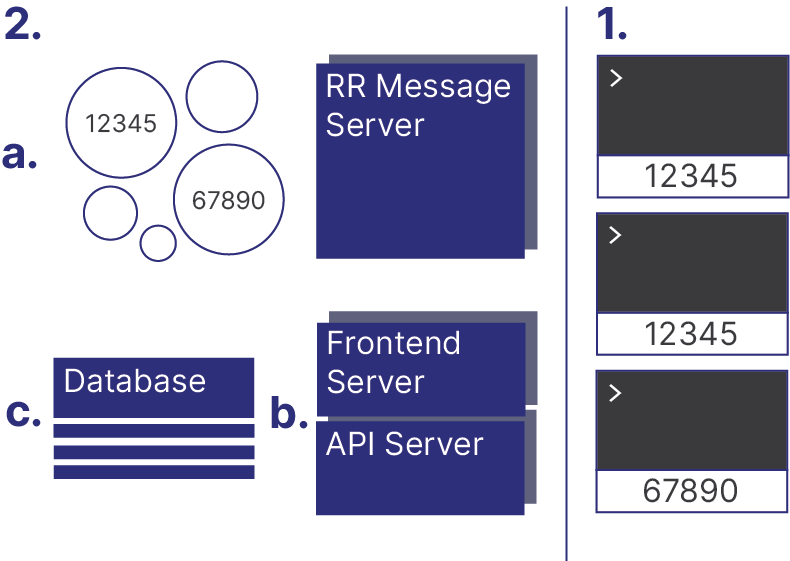
\includegraphics[scale=.8]{overall_system}
%   \centering
%   \caption{Overview of the Collaborative Debugger}
%   \label{debugger:overview}
% \end{figure}

% The next sections give an overview of the various tools used to create
% the collaborative debugger.  The debugger consists of:

% \begin{enumerate}
% \item A frontend web app built using React (\ref{react}) that presents
%   a debugging interface to the end user.
% \item A distributed backend managed by Kubernetes (\ref{k8s}), split
%   into three parts:
%   \begin{enumerate}
%   \item A Pod for each debugging instance which runs the rr debugger
%     (\ref{rr}).  These communicate directly with users through
%     WebSocket server Pods. (\ref{socketio}).
%   \item Pods running a frontend server written in Node.js which works
%     in tandem with an API server created using Flask
%     (\ref{flask/node}).  The API server manages creation and
%     destruction of debug sessions, as well as authentication.
%   \item A MongoDB (\ref{mongodb}) database.
%   \end{enumerate}
% \end{enumerate}

\section{Frontend/API Server}\label{api}

The second major backend system consists of the Frontend/API Server
and database.  This system is responsible for serving the frontend
webapp, as well as processing all API requests, such as those to
authenticate users and create new RR Debug Sessions.

\subsection{Tools Used}

\subsubsection{MongoDB}\label{mongodb}

The collaborative debugger uses a database to store information about
users, Pods, and example debugging sessions.  Due to it's speed of
deployment and natural interaction with the object-oriented languages
used to create the project, MongoDB was chosen as database software
\cite{mongodb}.

\subsubsection{Flask and Node.js}\label{flask/node}

The primary server for the collaborative debugger is split into two
sections: a simple Node.js \cite{node} server that serves the frontend
webapp, and an API server created using Flask \cite{flask}.  While in
development, the builtin React (\ref{react}) development server
is used to serve the frontend.  This makes debugging the frontend far
easier.
\par

An API server is necessary to authenticate users and to provide a
means to create/delete debugging sessions.  Since the rest of the
backend was created using Python, Flask was chosen to create the API
server.  Flask is a lightweight web application framework which lends
itself perfectly to interacting with the Python MongoDB and Kubernetes
APIs.

\subsection{Overview}

The builtin React development server is used to serve the frontend
webapp and redirect API requests to the Flask API server during
development.  For both security and performance reasons this should be
changed to a combination of a more robust solution like Nginx
\cite{nginx} and a production suitable web server for production.  The
relationships between components and overall process will remain
unchanged after this migration.
\par

Since the entire webapp is one page, the process for serving it is
completely standard.  The server receives a request for the index page
of the website, and returns the compiled React webapp that makes up
the homepage.  The process for API requests is more involved, and an
example is outlined below:

\begin{figure}[h!]

  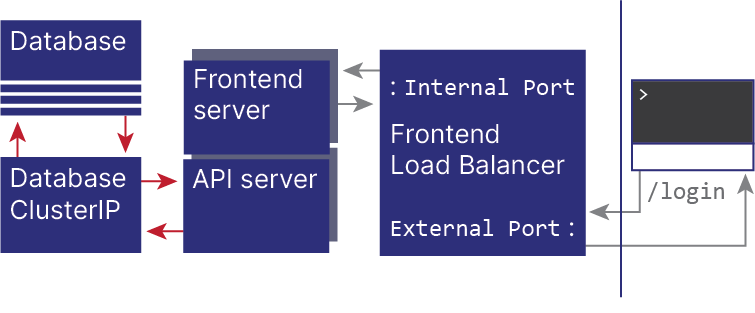
\includegraphics[scale=.9]{login_request}
  \centering
  \caption{API Request Process---Login}
  \label{rr:detailed}
\end{figure}

\begin{enumerate}
\item The client makes a POST request to the \lstinline{'/login'} URL.
  This request contains the necessary data to log in the user.
\item The frontend server forwards the request of a URL it does not
  recognize to the API server running in the same Pod on a different
  port.
\item The API server recognizes the \lstinline{'/login'} route, and
  communicates with the database to attempt to log in the user.
\item The API server returns the result of the login request, which is
  returned by the frontend server to the client.
\end{enumerate}

\subsection{Frontend/API Server Configuration}

The Frontend/API Server uses Yarn \cite{yarn} to manage packages.
When a Frontend/API Server Pod is deployed, the Pod's startup script
uses the \lstinline{yarn start} and \lstinline{yarn start-api}
commands to start the frontend server and API server respectively.
These scripts are defined in the server's \lstinline{package.json}
configuration file:

\begin{lstlisting}[basicstyle=\linespread{0.5}\ttfamily,caption={Frontend/API Server Configuration},captionpos=b]
  "start": "react-scripts start",
  "start-api": "cd api && flask run --no-debugger",
  .
  .
  .
  "proxy": "http://localhost:5000",
\end{lstlisting}

Also of note in \lstinline{package.json} is the instruction to proxy
the API server, which is running on port 5000.  This achieves the
automatic forwarding of API requests to the API server described
above.  Since API requests are proxied through the same address
serving the frontend webapp, there are no issues with cross-origin
requests.

\subsection{The API Server}

The API server is implemented using Flask.  The server program
consists of handlers for the various API routes and instances of two
classes which communicate with the database/Kubernetes API:
\lstinline{TranslationPodManager} and \lstinline{UserManager}.  The
full structure of the API Server program, \lstinline{api.py} is shown
below:

\begin{figure}[h!]

  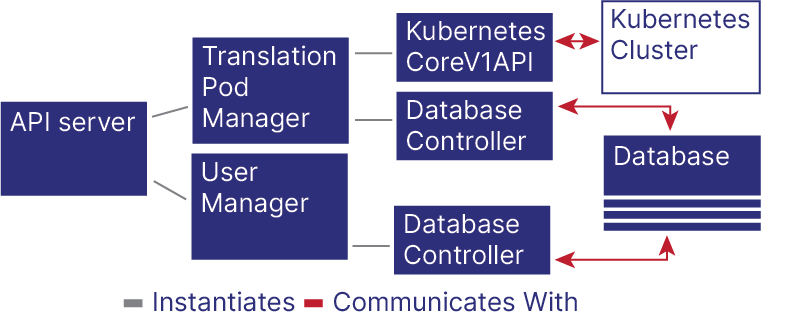
\includegraphics[scale=1]{api_structure}
  \centering
  \caption{Structure of the API Server}
  \label{rr:detailed}
\end{figure}

Care was taken to abstract as much as possible in the design of the
API server and the classes it instantiates.  The two classes
instantiated by \lstinline{api.py}, \lstinline{TranslationPodManager}
and \lstinline{UserManager}, each instantiate another class which
interacts with the database, \lstinline{DatabaseController}, as an
instance variable.  \lstinline{TranslationPodManager} further
instantiates the Kubernetes Core V1 Python API to communicate with the
cluster in order to create/delete pods.  This process of abstraction
ensures that the database, underlying cluster structure, and
authentication methods can all change without significant changes
needing to be made to \lstinline{api.py}.
\par

The most significant improvement that could be made to this structure
would be to break the \lstinline{UserManager} and
\lstinline{TranslationPodManager} instances out into separate programs
running on their own Pods in the cluster.  This would allow changes to
be made in those classes, say to update the process of deleting Pods,
without needing to update the entire Frontend/API Server Pod.  For the
time being, the relative simplicity of the API means that the added
complexity and overhead of implementing a method to communicate
between dedicated \lstinline{TranslationPodManager} and
\lstinline{UserManager} Pods and Pods running the Frontend/API Server
doesn't seem worthwhile.  This may change in the future.
\par

Currently supported API requests are as follows:

\begin{enumerate}
\item \lstinline{'/login'}: Logs in the user given by
  \lstinline{'name'}, or, (given the rather lax development security)
  creates a user if none matching \lstinline{'name'} exists.  Returns
  the name of the user.
\item \lstinline{'/channel'}: How users join RR Debug Sessions.  Binds
  the user given by \lstinline{'name'} to an RR Debug Session Pod
  matching \lstinline{'channel'} in the database, if such a Pod
  exists.  Returns the channel.
\item \lstinline{'/pods'}: How the client gets a list of RR Debug
  Session Pods the user is currently participating in.  Returns the
  channels for all RR Debug Session Pods who the user, given by
  \lstinline{'name'}, is currently bound to in the database.
\item \lstinline{'/examples}: How the client gets a list of example RR
  Debug Session Pod names.  Returns all names of example RR Debug
  Session Pods that exist in the database.
\item \lstinline{'/new'}: Creates a new RR Debug Session Pod based on
  the name given by \lstinline{'program'}.  Binds the user, given by
  \lstinline{'name'}, to the Pod.  Returns the channel of the Pod.
  This request is the most complex, and is covered in more detail
  below.
\item \lstinline{'/delete'}: Deletes a binding between the user given
  by \lstinline{'name'} and the RR Debug Session Pod given by
  \lstinline{'channel'}.  If there are no bindings left between the
  Pod and users (if all the users have left the debug session),
  deletes the Pod from the database and the cluster.  Returns
  \lstinline{True}.
\end{enumerate}

All the API request handlers listed above return an error message in
the case of an error occurring during the processing of an API
request.  Since most errors that could occur would either be the
result of unanticipated issues on the part of the user, or of some
unforeseen catastrophic internal error, informing users of error
specifics is often unhelpful.  Some \lstinline{TranslationPodManager}
and \lstinline{UserManager} functions throw specific errors in the
event of duplicate usernames, channels that do not exist, etc.  These
errors are caught and meaningful error messages are returned to the
frontend webapp, which can then pass them on to the user.
\par

To examine the process of processing an API request, it makes sense to
look at the most complex example, creating a new RR Debug Session Pod.
This example shows the process for processing an API POST request,
interacting with the database, and dynamically creating a Pod.  All
API requests follow a similar procedure.

\subsubsection{Processing a POST Request---Extracting Information}

Below is the route handler for the \lstinline{'/new'} URL, as well as
the instantiation of \lstinline{TranslationPodManager} and
\lstinline{UserManager}.

\begin{lstlisting}[language=Python,basicstyle=\linespread{0.5}\ttfamily,caption={API Server New RR Debug Session Event Handler},captionpos=b]
tpm = podmanager.TranslationPodManager(
                   url='mongodb://database-load-balancer',
                   port=27017)
um = usermanager.UserManager(
                   url='mongodb://database-load-balancer',
                   port=27017)
app = Flask(__name__)

@app.route('/new', methods=['POST'])
def new():
    try:
        name = request.get_json()['name']
        program = request.get_json()['program']
        channel = tpm.create_pod([name], program)
        return {'channel': channel}
    except:
        return {'error': 'Internal Error'}
\end{lstlisting}

All API routes only support POST requests.  The route handler first
extracts the relevant information from the POST request body, in this
case \lstinline{name} and \lstinline{program}.  \lstinline{name}
always corresponds the user who is making the request's username, and
\lstinline{program} corresponds to the name of the example RR Debug
Session image to be used.
\par

\lstinline{new} then calls \lstinline{TranslationPodManager}'s
\lstinline{create_pod} function to create a new RR Debug Session Pod.
\lstinline{create_pod} can bind multiple users to a Pod when it is
created, so \lstinline{name} is passed inside a list.

\subsubsection{The Database} Before drilling into \lstinline{create_pod},
it may be helpful to examine the MongoDB database which
\lstinline{TranslationPodManager} and \lstinline{UserManager} interact
with.  The database consists of three collections: \lstinline{users},
\lstinline{pods}, and \lstinline{examples}.  Below is an example
record from each collection:

\begin{figure}[h!]

  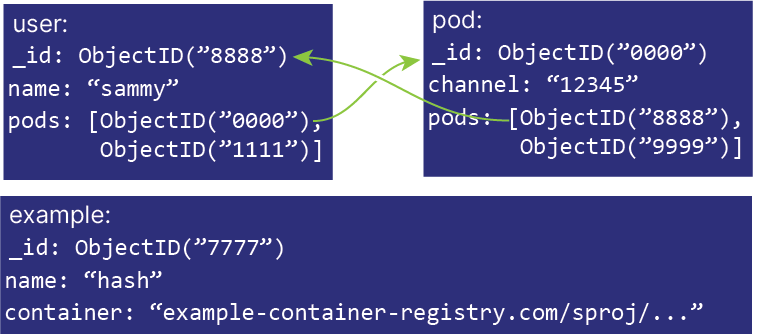
\includegraphics[scale=1]{database_example}
  \centering
  \caption{Database Record Examples}
  \label{rr:detailed}
\end{figure}

\lstinline{pods} and \lstinline{users} have a many-to-many
relationship.  Each user can be bound to an unlimited number of pods,
and vice versa.  The \lstinline{DatabaseController} class includes
functions to efficiently retrieve \lstinline{users} and
\lstinline{pods} given one another, and to create/destroy bindings
between \lstinline{users} and \lstinline{pods}.
\par

\lstinline{examples} are independent of \lstinline{users} and
\lstinline{pods}.  The container registry URLs of RR Debug Session
example images are stored in the database so that new images can be
easily added to the collaborative debugger upon creation.
\par

MongoDB keeps \lstinline{_id}s unique.  In addition, the collaborative
debugger defines uniqueness constrains on \lstinline{users.name},
\lstinline{pods.channel}, and \lstinline{examples.name} when the
database is created.

% \begin{lstlisting}[basicstyle=\linespread{0.5}\ttfamily,caption={Frontend/API Server Configuration},captionpos=b]
% users:            pods:               examples:
%   _id ObjectId      _id ObjectId        _id ObjectId
%   name String       channel String      name String
%   pods Array        users Array         container String

% Example user:
% {
% 	"_id" : ObjectId("5fc14c622dc45448d67189b3"),
% 	"name" : "sammy",
% 	"pods" : [
% 		ObjectId("5fc14d5b2dc45448d67189b4"),
% 		ObjectId("5fc59acb2dc45448d67189b6")
% 	]
% }

% Example pod:
% {
% 	"_id" : ObjectId("5fc14d5b2dc45448d67189b4"),
% 	"channel" : "19452",
% 	"users" : [
% 		ObjectId("5fc14c622dc45448d67189b3"),
% 		ObjectId("5fc317d22dc45448d67189b5")
% 	]
% }

% Example example:
% {
% 	"_id" : ObjectId("5fc14d50b92a752776d3fd7d"),
% 	"name" : "hash",
% 	"container" : "example-container-registry.com/sproj/..."
% }
% \end{lstlisting}

\subsubsection{Processing a POST Request---Dynamic Pod Creation} \label{dynamicc}

To dynamically create a Pod, \lstinline{create_pod} gets the container
registry URL of the image to base the Pod on, creates the new Pod,
binds users to the Pod, and returns the channel the Pod was created
with.  The first part of the function is shown below:

\begin{lstlisting}[language=Python,basicstyle=\linespread{0.5}\ttfamily,caption={Pod Creation 1},captionpos=b]
def create_pod(self, names, program):
  examples = self.get_examples()
  image = None
  try:
    image = examples[program]
  except:
    raise NoSuchExampleError
\end{lstlisting}

\lstinline{create_pod} calls \lstinline{TranslationPodManager}'s
\lstinline{get_examples} method to get a list of RR Debug Session
example image names and container registry URLs from the database.  In
the event that the user has somehow passed a spurious image name or has
passed a name when there are no images, an exception is raised.
Otherwise, a RR Debug Session Pod schema is created using the image:


\begin{lstlisting}[language=Python,basicstyle=\linespread{0.5}\ttfamily,caption={Pod Creation 2},captionpos=b]
  dep = {'apiVersion': 'v1',
         'kind': 'Pod',
         'metadata': {'labels':
                      {'purpose': 'translate-rr'}},
         'spec': {'containers':
                  [{'image': image,
                    'name': 'rr-test-container',
                    'command': ['sh'],
                    'args': ['startup.sh'],
                    'securityContext':
                    {'capabilities':
                     {'add': ['SYS_PTRACE']}}}],
                   'restartPolicy': 'OnFailure'}}
\end{lstlisting}

This schema, represented as a dictionary in Python, is identical to
the YAML representation of the RR Debug Session Pod creation schema
shown in (\ref{podschema}) with the exception of \lstinline{args}
which will be updated further in a later step.  Finally,
\lstinline{create_pod} does the
work necessary to dynamically create a Pod:

\begin{lstlisting}[language=Python,basicstyle=\linespread{0.5}\ttfamily,caption={Pod Creation 3},captionpos=b]
  channel = self.dbc.add_pod(
            self.dbc.get_userids_by_name(names))
  dep['metadata']['name'] = channel
  dep['spec']['containers'][0]['args'].append(channel)
  resp = self.v1.create_namespaced_pod(
         body=dep, namespace='default')
  # Wait to return the channel until the pod is live
  # and read to recieve incomming communication
  status = self.v1.read_namespaced_pod_status(
           channel, 'default').status.container_statuses
  while status == None or status[0].state.running == None:
    time.sleep(1)
    status = self.v1.read_namespaced_pod_status(
             channel, 'default').status.container_statuses
  return channel
\end{lstlisting}

First, \lstinline{DatabaseController}'s \lstinline{add_pod} method is
called to insert a new \lstinline{pods} record into the database.
\lstinline{add_pod} randomly generates a new five digit
\lstinline{channel} for the Pod, using the uniqueness constraint
imposed on \lstinline{pods.channel} to ensure an unused
\lstinline{channel} is generated.  If no channels are open an error is
raised.  Otherwise, the users passed to \lstinline{add_pod} are bound
to the new Pod in the database, and \lstinline{channel} is returned.
This process has the effect of limiting the number of simultaneous RR
Debug Sessions that can be in use at the same time to 89,999, and of
slowing as more channels are used.  Given the few current users, the
likelihood of a collision when generating a new channel is low enough
that a more advanced method is unnecessary.
\par

Next, the name of the container is updated to \lstinline{channel}.  In
addition, the startup arguments are updated to include
\lstinline{channel}.  This is how \lstinline{channel} is passed to the
\lstinline{startup.sh} script and eventually used to join a channel on
the RR Message Server in \lstinline{rrtranslation.py}
(\ref{buildingchannel} \& \ref{joiningchannel}).
\par

The Kubernetes API is then finally used to create the Pod.  The Pod is
created in the default namespace.  This could be changed to logically
isolate dynamically and statically created Pods with minimal hassle,
since Kubernetes' DNS resolution can connect pods across namespaces.
If Pod creation fails, an error will be thrown.  Otherwise, a loop is
used to wait until \lstinline{rrtranslation.py} is running inside the
Pod.  Once the Pod is ready, \lstinline{channel} is returned.

\subsubsection{Processing a POST Request---Returning a Response}

Most request handlers, \lstinline{'/new'} included, simply return a
JSON serializable dictionary containing whatever results the API
Server's instance of \lstinline{TranslationPodManager} or
\lstinline{UserManager} returned, or an error message.  The
\lstinline{'/new'} handler returns \lstinline{'channel': channel} so
that the frontend webapp's socket.io client can join the channel
corresponding to the RR Debug Session Pod that was just created.

\subsection{Considerations}

The Frontend/API server connects all components of the collaborative
debugger together.  It authenticates users through the database, joins
the frontend and Kubernetes cluster through the dynamic creation of
Pods, and starts the interaction between users and the programs they
wish to debug.  Care has been taken to make it modular and extensible
within reason, and additional authentication or pod creation features
should be easy to add.
\par

The experience provided by invisible components such as the
Frontend/API Server is just as important as that provided by the
frontend webapp.  All components of the collaborative debugger
hopefully come together to provide an experience that facilitates the
teaching and learning of debugging.

\section{Next Steps} \label{next}

\subsection{Current Functionality} \label{current}

The following section details the first few steps students take to
explore the \lstinline{memoization} example using the collaborative
debugger.  Students A and B begin by examining the call stack at its
deepest point in the recursive nth Fibonacci number function.  The
terminal interface to rr and the source code view have been
color-inverted to improve readability in this paper.

\begin{figure}[h!]

  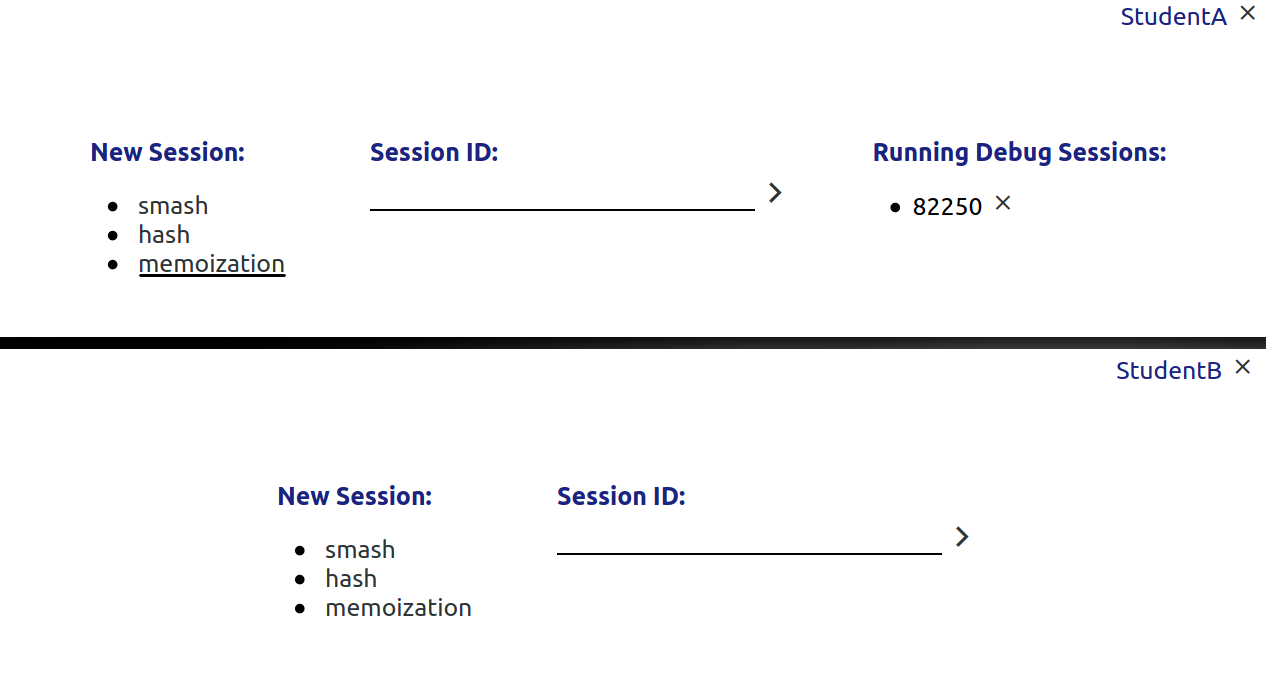
\includegraphics[width=\textwidth]{session1i}
  \centering
  \caption{Creating a new Memoization Example Session}
  \label{session1i}
\end{figure}

To start a new session, Student A selects ``memoization'' from the
list of example sessions.\pagebreak

\begin{figure}[h!]

  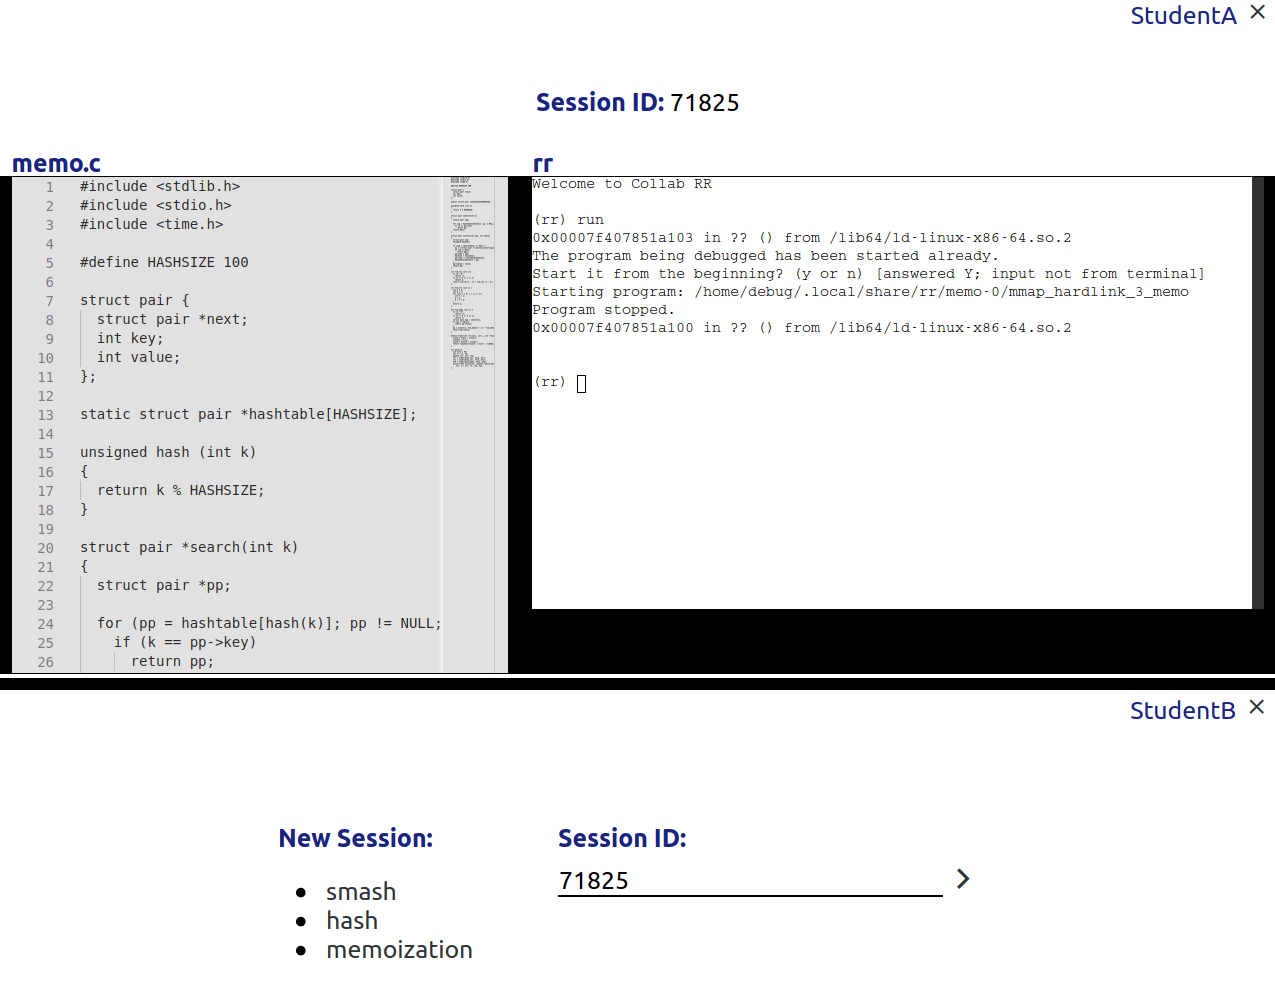
\includegraphics[width=\textwidth]{session2i}
  \centering
  \caption{Joining the Memoization Example Session}
  \label{session2i}
\end{figure}

In order to join Student A's session, Student B uses session code
``71825''.  Meanwhile, Student A is presented with the the main view
of the collaborative debugger.  On the right is a view of the source
code for the \lstinline{memoization} example.  On the left is the
terminal interface to rr.\pagebreak

\begin{figure}[h!]

  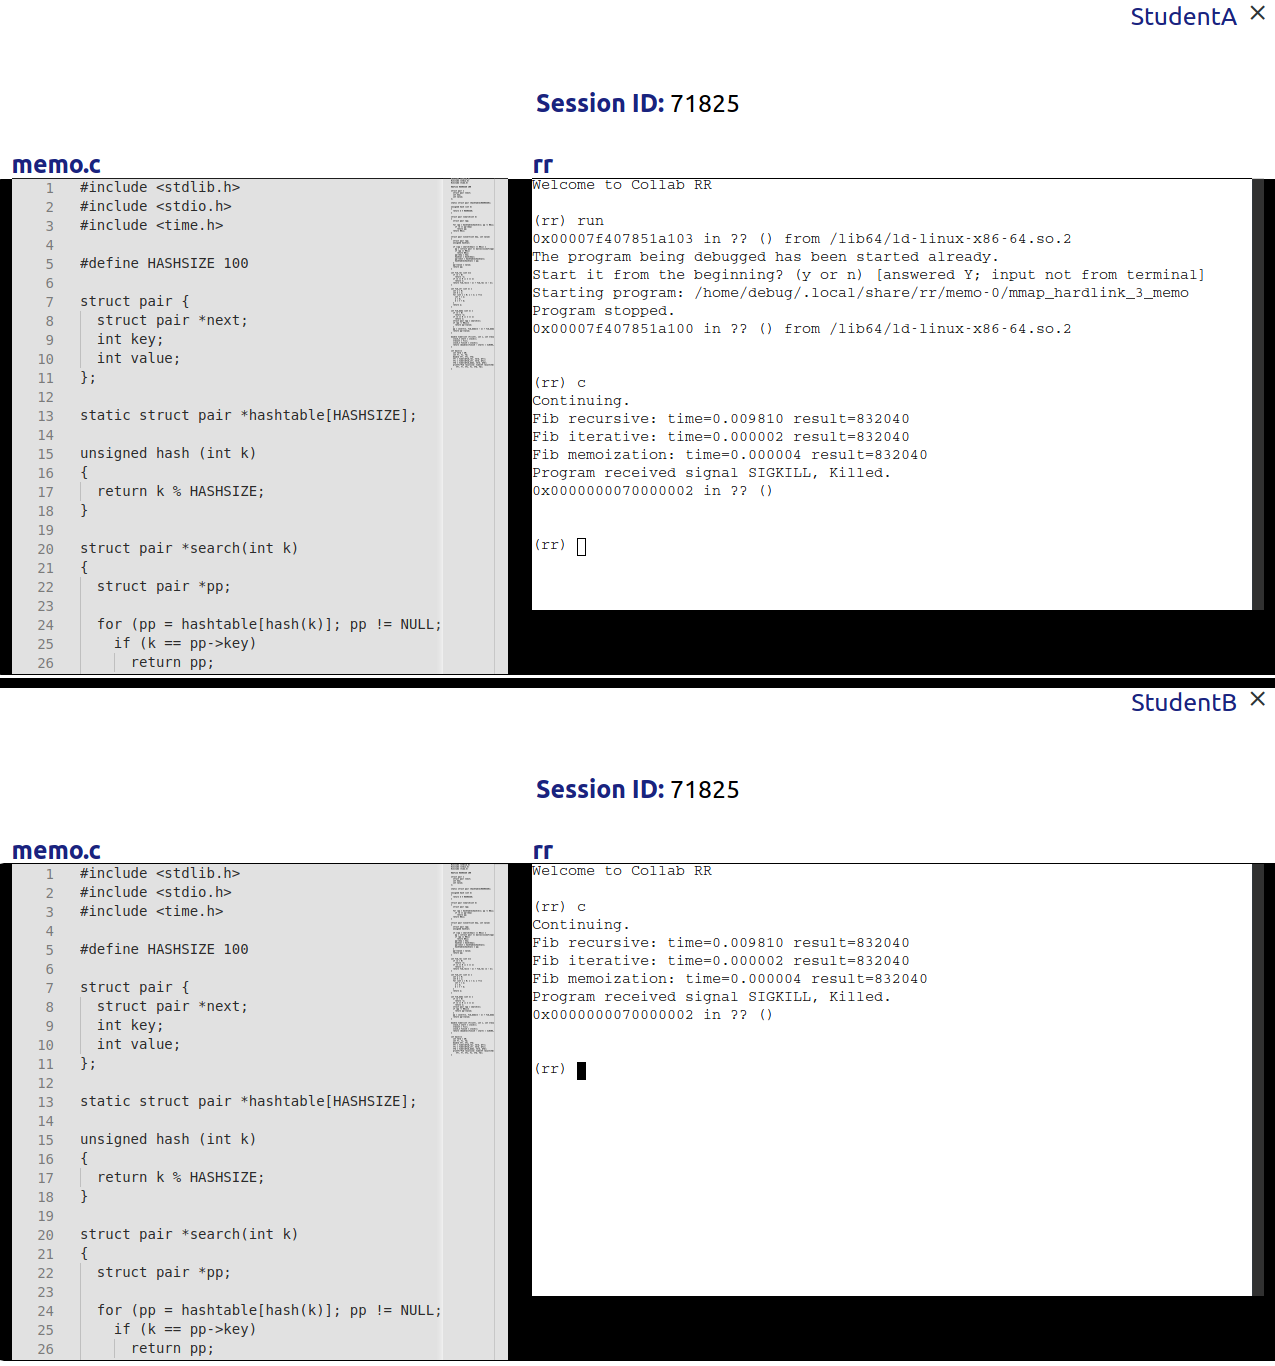
\includegraphics[width=\textwidth]{session3i}
  \centering
  \caption{Observing Output from the Memoization Example Session}
  \label{session3i}
\end{figure}

Student B now types \lstinline{c} to continue execution.  Both
students see the command and output: execution times and results for
three different implementations of nth Fibonacci.  An advantage of
rr's recording model is that these numbers will be the same every time
the students run the program.\pagebreak

\begin{figure}[h!]

  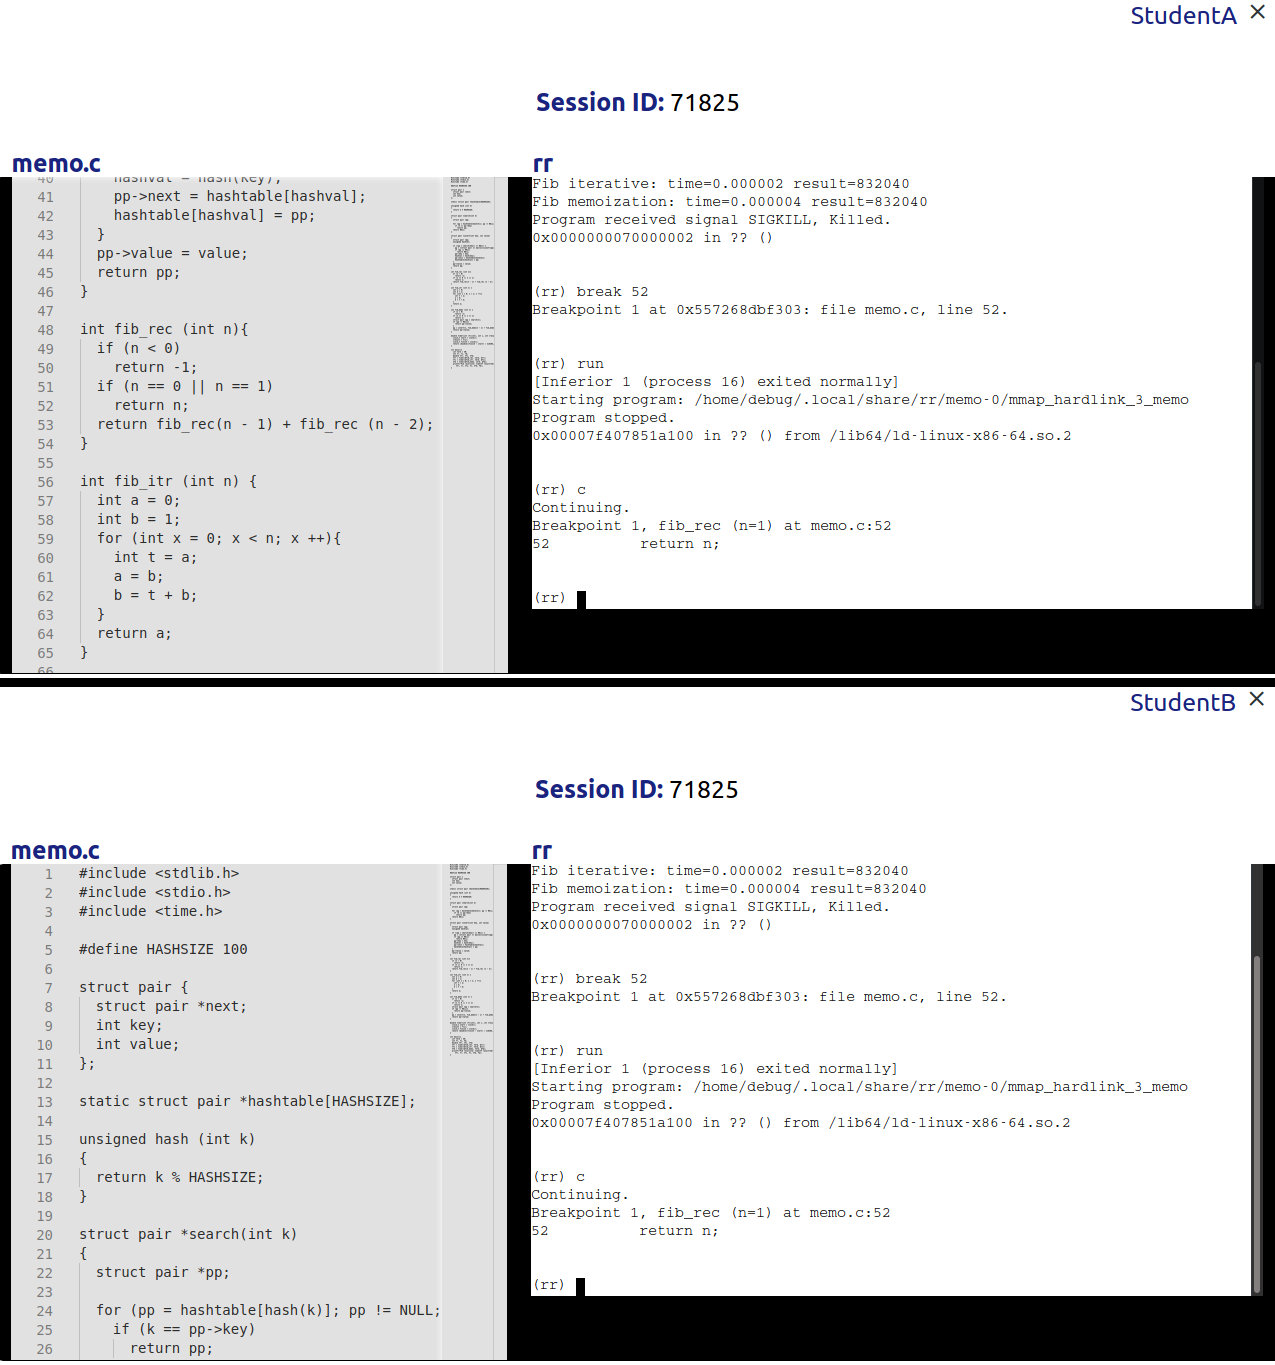
\includegraphics[width=\textwidth]{session4i}
  \centering
  \caption{Setting a Breakpoint in the Memoization Example Session}
  \label{session4i}
\end{figure}

Student A enters \lstinline{break 52} to set a breakpoint at line 52,
the base case of \lstinline{fib_rec}.  Student B types \lstinline{run}
and then \lstinline{c} to restart the recording and continue to the
breakpoint.\pagebreak

\begin{figure}[h!]

  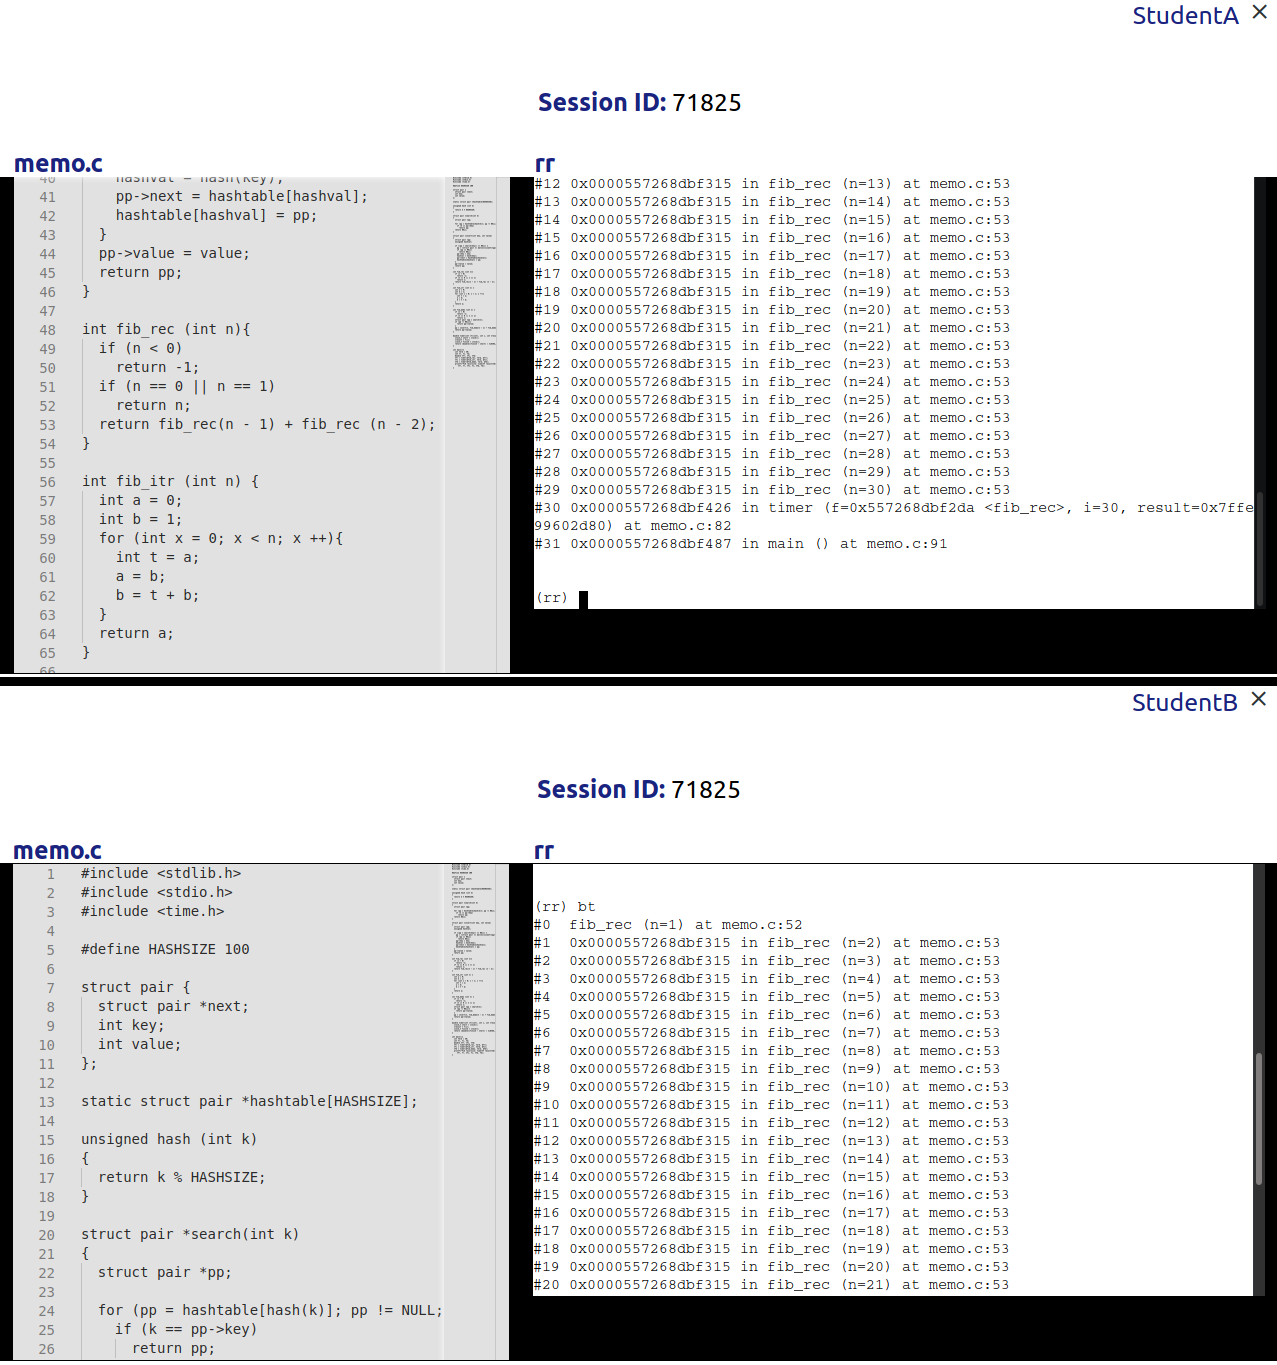
\includegraphics[width=\textwidth]{session5i}
  \centering
  \caption{Examining the Stack in the Memoization Example
    Session}
  \label{session5i}
\end{figure}

The students examine the stack resulting from a call of
\lstinline{fib_rec(30)}.  Students can inspect different areas of the
program and output while collaborating---Student A can look at
\lstinline{fib_rec}, while Student B scrolls up for a preview of the
memoized implementation.
\par

The students will continue to inspect the stack for other functions,
exploring the reasons for the vast performance disparity between
\lstinline{fib_memo} and \lstinline{fib_rec}.  Students A and B can
not only help each other to learn about the stack and memoization, but
can also teach one another how to use a debugger.  Because the
frontend produces near-identical output to rr, students can directly
translate their knowledge to it or gdb in the future.  Paradigms, such
as examining the stack to understand execution, can be expanded to all
future debugging.

\subsection{Features to Add}

The current iteration of the collaborative debugger successfully
enables collaboration between students.  Significant effort has been
taken to design the debugger in a way that makes collaboration
seamless.  The collaborative debugger hopefully fulfills it's first
requirement---to encourage collaboration.
\par

Though the collaborative debugger makes it easy for teachers to design
and distribute debugging lessons, more work is necessary to fully
fulfill the second goal---that of enhancing students' understanding of
debugging and of programs being debugged.
\par

The most significant addition towards this goal would be that of
frontend visualization tools.  A simple visualization of the stack and
registers would greatly expand students' understanding of the program
being debugged in all three example sessions currently included with
the collaborative debugger.  gdb/mi supports commands which give
structured output of both these aspects of the execution space, and
the frontend has been designed to make adding visualizations of them
simple.  Adding visualization features will bring the collaborative
debugger much closer towards hopefully fulfilling it's second
requirement.

\subsection{Testing Efficacy}

Though a review of the research seems to indicate that a tool like the
collaborative debugger should help make students more effective at
debugging, further study is needed to draw conclusions.  First, more
research is necessary to determine definitively if teaching debugging
collaboratively is more effective than teaching it individually.
Second, the collaborative debugger needs to be thoroughly tested to
determine whether it is an ideal platform for collaborative debugging.
\par

A study similar to those undertaken in \cite{10.1145/1026487.1008043},
\cite{10.1145/1145287.1145293}, and \cite{10.1145/3361721.3361724}
could be done to test both these aspects.  Students participating in
an introductory systems programming class could be split into three
groups.  Group one could study debugging individually, using rr by
themselves to progress through debugging sessions designed by the
instructor.  Group two could study debugging in pairs, relying on
existing tools such as video-conferencing software to facilitate
collaboration.  In the final group, pairs would use the collaborative
debugger to work together on the same debugging sessions as groups one
and two.  Students' individual and pair performance in debugging both
unseen and self-generated programs could then be tested.

\subsection{Conclusions}

The collaborative debugger aims to encourage collaboration and build
students knowledge of debugging through careful design.  Many
components of a distributed system come together to create a platform
that hopefully benefits both teachers and students.  Through
deliberate design, the collaborative debugger can conceivably be the
ideal platform to teach and learn debugging, both remotely and
in-person.

\pagebreak
\bibliographystyle{acm}
\bibliography{sprojbib}{}
\end{document}
